\documentclass[times, doublespace]{simauth}\usepackage[]{graphicx}\usepackage[]{color}
%% maxwidth is the original width if it is less than linewidth
%% otherwise use linewidth (to make sure the graphics do not exceed the margin)
\makeatletter
\def\maxwidth{ %
  \ifdim\Gin@nat@width>\linewidth
    \linewidth
  \else
    \Gin@nat@width
  \fi
}
\makeatother

\definecolor{fgcolor}{rgb}{0.345, 0.345, 0.345}
\newcommand{\hlnum}[1]{\textcolor[rgb]{0.686,0.059,0.569}{#1}}%
\newcommand{\hlstr}[1]{\textcolor[rgb]{0.192,0.494,0.8}{#1}}%
\newcommand{\hlcom}[1]{\textcolor[rgb]{0.678,0.584,0.686}{\textit{#1}}}%
\newcommand{\hlopt}[1]{\textcolor[rgb]{0,0,0}{#1}}%
\newcommand{\hlstd}[1]{\textcolor[rgb]{0.345,0.345,0.345}{#1}}%
\newcommand{\hlkwa}[1]{\textcolor[rgb]{0.161,0.373,0.58}{\textbf{#1}}}%
\newcommand{\hlkwb}[1]{\textcolor[rgb]{0.69,0.353,0.396}{#1}}%
\newcommand{\hlkwc}[1]{\textcolor[rgb]{0.333,0.667,0.333}{#1}}%
\newcommand{\hlkwd}[1]{\textcolor[rgb]{0.737,0.353,0.396}{\textbf{#1}}}%
\let\hlipl\hlkwb

\usepackage{framed}
\makeatletter
\newenvironment{kframe}{%
 \def\at@end@of@kframe{}%
 \ifinner\ifhmode%
  \def\at@end@of@kframe{\end{minipage}}%
  \begin{minipage}{\columnwidth}%
 \fi\fi%
 \def\FrameCommand##1{\hskip\@totalleftmargin \hskip-\fboxsep
 \colorbox{shadecolor}{##1}\hskip-\fboxsep
     % There is no \\@totalrightmargin, so:
     \hskip-\linewidth \hskip-\@totalleftmargin \hskip\columnwidth}%
 \MakeFramed {\advance\hsize-\width
   \@totalleftmargin\z@ \linewidth\hsize
   \@setminipage}}%
 {\par\unskip\endMakeFramed%
 \at@end@of@kframe}
\makeatother

\definecolor{shadecolor}{rgb}{.97, .97, .97}
\definecolor{messagecolor}{rgb}{0, 0, 0}
\definecolor{warningcolor}{rgb}{1, 0, 1}
\definecolor{errorcolor}{rgb}{1, 0, 0}
\newenvironment{knitrout}{}{} % an empty environment to be redefined in TeX

\usepackage{alltt}
%\documentclass[times]{simauth}
%\documentclass[]{article}

%\articletype{Article Type}%

%\received{}
%\revised{}
%\accepted{}

%\raggedbottom

%\usepackage[top=1in, bottom=1.25in, left=1.25in, right=1.25in]{geometry}

%\usepackage[colorlinks=true, urlcolor=citecolor, linkcolor=citecolor, citecolor=citecolor]{hyperref}

% Add history information for the article if required
%\history{Received August 1, 2010;
%revised October 1, 2010;
%accepted for publication November 1, 2010}

\usepackage{amssymb, amsmath, amsfonts}
%\usepackage{amsrefs}
\usepackage{color}
\usepackage[list=off]{caption} % list=off option prevents errors when using math environments within captions
%\usepackage{natbib}
%\usepackage{cite}

%%%%%%%%%%%%%%%%%%%%%%%%%%%%%%%%%%%%%%%%%%%%%%
%                                            %
%        GrandMacros.tex                     %
%                                            %
%  A file containing all non-colour LaTeX    %
%  macros used by M.P. Wand                  %
%                                            %
%     Last changed: 18th Oct, 2000           %
%                                            %
%%%%%%%%%%%%%%%%%%%%%%%%%%%%%%%%%%%%%%%%%%%%%%
%
% Conventions (for most current macros):
%
% \ba        <-->  bold-faced a
% \ahat      <-->  hatted a
% \atilde    <-->  tilded a
% \abar      <-->  barred a
% \asc       <-->  script a
% \aarrow    <-->  arrowed a
% \smbalpha  <-->  small bold-faced alpha
%
%%%%%%%%%%%%%%%%%%%%%%%%%%
%  Bold Digits           %
%%%%%%%%%%%%%%%%%%%%%%%%%%
%
%
\def\bzero{{\bf 0}}
\def\bone{{\bf 1}}
%
%
%%%%%%%%%%%%%%%%%%%%%%%%%%
%  Bold Roman Letters    %
%%%%%%%%%%%%%%%%%%%%%%%%%%
%
%
\def\ba{{\mbox{\boldmath$a$}}}
\def\bb{{\bf b}}
\def\bc{{\bf c}}
\def\bd{{\bf d}}
\def\be{{\bf e}}
\def\bdf{{\bf f}}
\def\bg{{\mbox{\boldmath$g$}}}
\def\bh{{\bf h}}
\def\bi{{\bf i}}
\def\bj{{\bf j}}
\def\bk{{\bf k}}
\def\bl{{\bf l}}
\def\bm{{\bf m}}
\def\bn{{\bf n}}
\def\bo{{\bf o}}
\def\bp{{\bf p}}
\def\bq{{\bf q}}
\def\br{{\bf r}}
\def\bs{{\bf s}}
\def\bt{{\bf t}}
\def\bu{{\bf u}}
\def\bv{{\bf v}}
\def\bw{{\bf w}}
\def\bx{{\bf x}}
\def\by{{\bf y}}
\def\bz{{\bf z}}
\def\bA{{\bf A}}
\def\bB{{\bf B}}
\def\bC{{\bf C}}
\def\bD{{\bf D}}
\def\bE{{\bf E}}
\def\bF{{\bf F}}
\def\bG{{\bf G}}
\def\bH{{\bf H}}
\def\bI{{\bf I}}
\def\bJ{{\bf J}}
\def\bK{{\bf K}}
\def\bL{{\bf L}}
\def\bM{{\bf M}}
\def\bN{{\bf N}}
\def\bO{{\bf O}}
\def\bP{{\bf P}}
\def\bQ{{\bf Q}}
\def\bR{{\bf R}}
\def\bS{{\bf S}}
\def\bT{{\bf T}}
\def\bU{{\bf U}}
\def\bV{{\bf V}}
\def\bW{{\bf W}}
\def\bX{{\bf X}}
\def\bY{{\bf Y}}
\def\bZ{{\bf Z}}
%
%
%%%%%%%%%%%%%%%%%%%%%%%%%%
%  Bold Greek Letters    %
%%%%%%%%%%%%%%%%%%%%%%%%%%
%
%
\def\thick#1{\hbox{\rlap{$#1$}\kern0.25pt\rlap{$#1$}\kern0.25pt$#1$}}
\def\balpha{{\thick\alpha}}
\def\bbeta{{\thick\beta}}
\def\bgamma{{\thick\gamma}}
\def\bdelta{{\thick\delta}}
\def\bepsilon{{\thick\epsilon}}
\def\bvarepsilon{{\thick\varepsilon}}
\def\bzeta{{\thick\zeta}}
\def\bdeta{{\thick\eta}}
\def\btheta{{\thick\theta}}
\def\biota{{\thick\iota}}
\def\bkappa{{\thick\kappa}}
\def\blambda{{\thick\lambda}}
\def\bmu{{\thick\mu}}
\def\bnu{{\thick\nu}}
\def\bxi{{\thick\xi}}
\def\bomicron{{\thick\omicron}}
\def\bpi{{\thick\pi}}
\def\brho{{\thick\rho}}
\def\bsigma{{\thick\sigma}}
\def\btau{{\thick\tau}}
\def\bupsilon{{\thick\upsilon}}
\def\bphi{{\thick\phi}}
\def\bchi{{\thick\chi}}
\def\bpsi{{\thick\psi}}
\def\bomega{{\thick\omega}}
\def\bAlpha{{\thick\Alpha}}
\def\bBeta{{\thick\Beta}}
\def\bGamma{{\thick\Gamma}}
\def\bDelta{{\thick\Delta}}
\def\bEpsilon{{\thick\Epsilon}}
\def\bZeta{{\thick\Zeta}}
\def\bEta{{\thick\Eta}}
\def\bTheta{{\thick\Theta}}
\def\bIota{{\thick\Iota}}
\def\bKappa{{\thick\Kappa}}
\def\bLambda{{\thick\Lambda}}
\def\bMu{{\thick\Mu}}
\def\bNu{{\thick\Nu}}
\def\bXi{{\thick\Xi}}
\def\bOmicron{{\thick\Omicron}}
\def\bPi{{\thick\Pi}}
\def\bRho{{\thick\Rho}}
\def\bSigma{{\thick\Sigma}}
\def\bTau{{\thick\Tau}}
\def\bUpsilon{{\thick\Upsilon}}
\def\bPhi{{\thick\Phi}}
\def\bChi{{\thick\Chi}}
\def\bPsi{{\thick\Psi}}
\def\bOmega{{\thick\Omega}}
%
%
%
%%%%%%%%%%%%%%%%%%%%%%%%%%%%%%%%
%  Small Bold Greek Letters    %
%%%%%%%%%%%%%%%%%%%%%%%%%%%%%%%%
\def\smbalpha{{\thick{\scriptstyle{\alpha}}}}
\def\smbbeta{{\thick{\scriptstyle{\beta}}}}
\def\smbgamma{{\thick{\scriptstyle{\gamma}}}}
\def\smbdelta{{\thick{\scriptstyle{\delta}}}}
\def\smbepsilon{{\thick{\scriptstyle{\epsilon}}}}
\def\smbvarepsilon{{\thick{\scriptstyle{\varepsilon}}}}
\def\smbzeta{{\thick{\scriptstyle{\zeta}}}}
\def\smbdeta{{\thick{\scriptstyle{\eta}}}}
\def\smbtheta{{\thick{\scriptstyle{\theta}}}}
\def\smbiota{{\thick{\scriptstyle{\iota}}}}
\def\smbkappa{{\thick{\scriptstyle{\kappa}}}}
\def\smblambda{{\thick{\scriptstyle{\lambda}}}}
\def\smbmu{{\thick{\scriptstyle{\mu}}}}
\def\smbnu{{\thick{\scriptstyle{\nu}}}}
\def\smbxi{{\thick{\scriptstyle{\xi}}}}
\def\smbomicron{{\thick{\scriptstyle{\omicron}}}}
\def\smbpi{{\thick{\scriptstyle{\pi}}}}
\def\smbrho{{\thick{\scriptstyle{\rho}}}}
\def\smbsigma{{\thick{\scriptstyle{\sigma}}}}
\def\smbtau{{\thick{\scriptstyle{\tau}}}}
\def\smbupsilon{{\thick{\scriptstyle{\upsilon}}}}
\def\smbphi{{\thick{\scriptstyle{\phi}}}}
\def\smbchi{{\thick{\scriptstyle{\chi}}}}
\def\smbpsi{{\thick{\scriptstyle{\psi}}}}
\def\smbomega{{\thick{\scriptstyle{\omega}}}}
\def\smbAlpha{{\thick{\scriptstyle{\Alpha}}}}
\def\smbBeta{{\thick{\scriptstyle{\Beta}}}}
\def\smbGamma{{\thick{\scriptstyle{\Gamma}}}}
\def\smbDelta{{\thick{\scriptstyle{\Delta}}}}
\def\smbEpsilon{{\thick{\scriptstyle{\Epsilon}}}}
\def\smbZeta{{\thick{\scriptstyle{\Zeta}}}}
\def\smbEta{{\thick{\scriptstyle{\Eta}}}}
\def\smbTheta{{\thick{\scriptstyle{\Theta}}}}
\def\smbIota{{\thick{\scriptstyle{\Iota}}}}
\def\smbKappa{{\thick{\scriptstyle{\Kappa}}}}
\def\smbLambda{{\thick{\scriptstyle{\Lambda}}}}
\def\smbMu{{\thick{\scriptstyle{\Mu}}}}
\def\smbNu{{\thick{\scriptstyle{\Nu}}}}
\def\smbXi{{\thick{\scriptstyle{\Xi}}}}
\def\smbOmicron{{\thick{\scriptstyle{\Omicron}}}}
\def\smbPi{{\thick{\scriptstyle{\Pi}}}}
\def\smbRho{{\thick{\scriptstyle{\Rho}}}}
\def\smbSigma{{\thick{\scriptstyle{\Sigma}}}}
\def\smbTau{{\thick{\scriptstyle{\Tau}}}}
\def\smbUpsilon{{\thick{\scriptstyle{\Upsilon}}}}
\def\smbPhi{{\thick{\scriptstyle{\Phi}}}}
\def\smbChi{{\thick{\scriptstyle{\Chi}}}}
\def\smbPsi{{\thick{\scriptstyle{\Psi}}}}
\def\smbOmega{{\thick{\scriptstyle{\Omega}}}}
%
%
%%%%%%%%%%%%%%%%%%%%%%%%%%
%  Hatted Roman Letters  %
%%%%%%%%%%%%%%%%%%%%%%%%%%
%
%
\def\ahat{{\widehat a}}
\def\bhat{{\widehat b}}
\def\chat{{\widehat c}}
\def\dhat{{\widehat d}}
\def\ehat{{\widehat e}}
\def\fhat{{\widehat f}}
\def\ghat{{\widehat g}}
\def\hhat{{\widehat h}}
\def\ihat{{\widehat i}}
\def\jhat{{\widehat j}}
\def\khat{{\widehat k}}
\def\lhat{{\widehat l}}
\def\mhat{{\widehat m}}
\def\nhat{{\widehat n}}
\def\ohat{{\widehat o}}
\def\phat{{\widehat p}}
\def\qhat{{\widehat q}}
\def\rhat{{\widehat r}}
\def\shat{{\widehat s}}
\def\that{{\widehat t}}
\def\uhat{{\widehat u}}
\def\vhat{{\widehat v}}
\def\what{{\widehat w}}
\def\xhat{{\widehat x}}
\def\yhat{{\widehat y}}
\def\zhat{{\widehat z}}
\def\Ahat{{\widehat A}}
\def\Bhat{{\widehat B}}
\def\Chat{{\widehat C}}
\def\Dhat{{\widehat D}}
\def\Ehat{{\widehat E}}
\def\Fhat{{\widehat F}}
\def\Ghat{{\widehat G}}
\def\Hhat{{\widehat H}}
\def\Ihat{{\widehat I}}
\def\Jhat{{\widehat J}}
\def\Khat{{\widehat K}}
\def\Lhat{{\widehat L}}
\def\Mhat{{\widehat M}}
\def\Nhat{{\widehat N}}
\def\Ohat{{\widehat O}}
\def\Phat{{\widehat P}}
\def\Qhat{{\widehat Q}}
\def\Rhat{{\widehat R}}
\def\Shat{{\widehat S}}
\def\That{{\widehat T}}
\def\Uhat{{\widehat U}}
\def\Vhat{{\widehat V}}
\def\What{{\widehat W}}
\def\Xhat{{\widehat X}}
\def\Yhat{{\widehat Y}}
\def\Zhat{{\widehat Z}}
%
%%%%%%%%%%%%%%%%%%%%%%%%%%
%  Tilded Roman Letters  %
%%%%%%%%%%%%%%%%%%%%%%%%%%
%
%
\def\atilde{{\widetilde a}}
\def\btilde{{\widetilde b}}
\def\ctilde{{\widetilde c}}
\def\dtilde{{\widetilde d}}
\def\etilde{{\widetilde e}}
\def\ftilde{{\widetilde f}}
\def\gtilde{{\widetilde g}}
\def\htilde{{\widetilde h}}
\def\itilde{{\widetilde i}}
\def\jtilde{{\widetilde j}}
\def\ktilde{{\widetilde k}}
\def\ltilde{{\widetilde l}}
\def\mtilde{{\widetilde m}}
\def\ntilde{{\widetilde n}}
\def\otilde{{\widetilde o}}
\def\ptilde{{\widetilde p}}
\def\qtilde{{\widetilde q}}
\def\rtilde{{\widetilde r}}
\def\stilde{{\widetilde s}}
\def\ttilde{{\widetilde t}}
\def\utilde{{\widetilde u}}
\def\vtilde{{\widetilde v}}
\def\wtilde{{\widetilde w}}
\def\xtilde{{\widetilde x}}
\def\ytilde{{\widetilde y}}
\def\ztilde{{\widetilde z}}
\def\Atilde{{\widetilde A}}
\def\Btilde{{\widetilde B}}
\def\Ctilde{{\widetilde C}}
\def\Dtilde{{\widetilde D}}
\def\Etilde{{\widetilde E}}
\def\Ftilde{{\widetilde F}}
\def\Gtilde{{\widetilde G}}
\def\Htilde{{\widetilde H}}
\def\Itilde{{\widetilde I}}
\def\Jtilde{{\widetilde J}}
\def\Ktilde{{\widetilde K}}
\def\Ltilde{{\widetilde L}}
\def\Mtilde{{\widetilde M}}
\def\Ntilde{{\widetilde N}}
\def\Otilde{{\widetilde O}}
\def\Ptilde{{\widetilde P}}
\def\Qtilde{{\widetilde Q}}
\def\Rtilde{{\widetilde R}}
\def\Stilde{{\widetilde S}}
\def\Ttilde{{\widetilde T}}
\def\Utilde{{\widetilde U}}
\def\Vtilde{{\widetilde V}}
\def\Wtilde{{\widetilde W}}
\def\Xtilde{{\widetilde X}}
\def\Ytilde{{\widetilde Y}}
\def\Ztilde{{\widetilde Z}}
%
%
%%%%%%%%%%%%%%%%%%%%%%%%%%%%%%%%%%%%
%  Hatted Bold-faced Roman Letters %
%%%%%%%%%%%%%%%%%%%%%%%%%%%%%%%%%%%%
%
%
\def\bahat{{\widehat \ba}}
\def\bbhat{{\widehat \bb}}
\def\bchat{{\widehat \bc}}
\def\bdhat{{\widehat \bd}}
\def\behat{{\widehat \be}}
\def\bfhat{{\widehat \bf}}
\def\bghat{{\widehat \bg}}
\def\bhhat{{\widehat \bh}}
\def\bihat{{\widehat \bi}}
\def\bjhat{{\widehat \bj}}
\def\bkhat{{\widehat \bk}}
\def\blhat{{\widehat \bl}}
\def\bmhat{{\widehat \bm}}
\def\bnhat{{\widehat \bn}}
\def\bohat{{\widehat \bo}}
\def\bphat{{\widehat \bp}}
\def\bqhat{{\widehat \bq}}
\def\brhat{{\widehat \br}}
\def\bshat{{\widehat \bs}}
\def\bthat{{\widehat \bt}}
\def\buhat{{\widehat \bu}}
\def\bvhat{{\widehat \bv}}
\def\bwhat{{\widehat \bw}}
\def\bxhat{{\widehat \bx}}
\def\byhat{{\widehat \by}}
\def\bzhat{{\widehat \bz}}
\def\bAhat{{\widehat \bA}}
\def\bBhat{{\widehat \bB}}
\def\bChat{{\widehat \bC}}
\def\bDhat{{\widehat \bD}}
\def\bEhat{{\widehat \bE}}
\def\bFhat{{\widehat \bF}}
\def\bGhat{{\widehat \bG}}
\def\bHhat{{\widehat \bH}}
\def\bIhat{{\widehat \bI}}
\def\bJhat{{\widehat \bJ}}
\def\bKhat{{\widehat \bK}}
\def\bLhat{{\widehat \bL}}
\def\bMhat{{\widehat \bM}}
\def\bNhat{{\widehat \bN}}
\def\bOhat{{\widehat \bO}}
\def\bPhat{{\widehat \bP}}
\def\bQhat{{\widehat \bQ}}
\def\bRhat{{\widehat \bR}}
\def\bShat{{\widehat \bS}}
\def\bThat{{\widehat \bT}}
\def\bUhat{{\widehat \bU}}
\def\bVhat{{\widehat \bV}}
\def\bWhat{{\widehat \bW}}
\def\bXhat{{\widehat \bX}}
\def\bYhat{{\widehat \bY}}
\def\bZhat{{\widehat \bZ}}
%
%
%
%%%%%%%%%%%%%%%%%%%%%%%%%%%%%%%%%%%%
%  Tilded Bold-faced Roman Letters %
%%%%%%%%%%%%%%%%%%%%%%%%%%%%%%%%%%%%
%
%
\def\batilde{{\widetilde \ba}}
\def\bbtilde{{\widetilde \bb}}
\def\bctilde{{\widetilde \bc}}
\def\bdtilde{{\widetilde \bd}}
\def\betilde{{\widetilde \be}}
\def\bftilde{{\widetilde \bf}}
\def\bgtilde{{\widetilde \bg}}
\def\bhtilde{{\widetilde \bh}}
\def\bitilde{{\widetilde \bi}}
\def\bjtilde{{\widetilde \bj}}
\def\bktilde{{\widetilde \bk}}
\def\bltilde{{\widetilde \bl}}
\def\bmtilde{{\widetilde \bm}}
\def\bntilde{{\widetilde \bn}}
\def\botilde{{\widetilde \bo}}
\def\bptilde{{\widetilde \bp}}
\def\bqtilde{{\widetilde \bq}}
\def\brtilde{{\widetilde \br}}
\def\bstilde{{\widetilde \bs}}
\def\bttilde{{\widetilde \bt}}
\def\butilde{{\widetilde \bu}}
\def\bvtilde{{\widetilde \bv}}
\def\bwtilde{{\widetilde \bw}}
\def\bxtilde{{\widetilde \bx}}
\def\bytilde{{\widetilde \by}}
\def\bztilde{{\widetilde \bz}}
\def\bAtilde{{\widetilde \bA}}
\def\bBtilde{{\widetilde \bB}}
\def\bCtilde{{\widetilde \bC}}
\def\bDtilde{{\widetilde \bD}}
\def\bEtilde{{\widetilde \bE}}
\def\bFtilde{{\widetilde \bF}}
\def\bGtilde{{\widetilde \bG}}
\def\bHtilde{{\widetilde \bH}}
\def\bItilde{{\widetilde \bI}}
\def\bJtilde{{\widetilde \bJ}}
\def\bKtilde{{\widetilde \bK}}
\def\bLtilde{{\widetilde \bL}}
\def\bMtilde{{\widetilde \bM}}
\def\bNtilde{{\widetilde \bN}}
\def\bOtilde{{\widetilde \bO}}
\def\bPtilde{{\widetilde \bP}}
\def\bQtilde{{\widetilde \bQ}}
\def\bRtilde{{\widetilde \bR}}
\def\bStilde{{\widetilde \bS}}
\def\bTtilde{{\widetilde \bT}}
\def\bUtilde{{\widetilde \bU}}
\def\bVtilde{{\widetilde \bV}}
\def\bWtilde{{\widetilde \bW}}
\def\bXtilde{{\widetilde \bX}}
\def\bYtilde{{\widetilde \bY}}
\def\bZtilde{{\widetilde \bZ}}
%
%
%
%
%%%%%%%%%%%%%%%%%%%%%%%%%%
%  Hatted Greek Letters  %
%%%%%%%%%%%%%%%%%%%%%%%%%%
%
%
\def\alphahat{{\widehat\alpha}}
\def\betahat{{\widehat\beta}}
\def\gammahat{{\widehat\gamma}}
\def\deltahat{{\widehat\delta}}
\def\epsilonhat{{\widehat\epsilon}}
\def\varepsilonhat{{\widehat\varepsilon}}
\def\zetahat{{\widehat\zeta}}
\def\etahat{{\widehat\eta}}
\def\thetahat{{\widehat\theta}}
\def\iotahat{{\widehat\iota}}
\def\kappahat{{\widehat\kappa}}
\def\lambdahat{{\widehat\lambda}}
\def\muhat{{\widehat\mu}}
\def\nuhat{{\widehat\nu}}
\def\xihat{{\widehat\xi}}
\def\omicronhat{{\widehat\omicron}}
\def\pihat{{\widehat\pi}}
\def\rhohat{{\widehat\rho}}
\def\sigmahat{{\widehat\sigma}}
\def\tauhat{{\widehat\tau}}
\def\upsilonhat{{\widehat\upsilon}}
\def\phihat{{\widehat\phi}}
\def\chihat{{\widehat\chi}}
\def\psihat{{\widehat\psi}}
\def\omegahat{{\widehat\omega}}
\def\Alphahat{{\widehat\Alpha}}
\def\Betahat{{\widehat\Beta}}
\def\Gammahat{{\widehat\Gamma}}
\def\Deltahat{{\widehat\Delta}}
\def\Epsilonhat{{\widehat\Epsilon}}
\def\Zetahat{{\widehat\Zeta}}
\def\Etahat{{\widehat\Eta}}
\def\Thetahat{{\widehat\Theta}}
\def\Iotahat{{\widehat\Iota}}
\def\Kappahat{{\widehat\Kappa}}
\def\Lambdahat{{\widehat\Lambda}}
\def\Muhat{{\widehat\Mu}}
\def\Nuhat{{\widehat\Nu}}
\def\Xihat{{\widehat\Xi}}
\def\Omicronhat{{\widehat\Omicron}}
\def\Pihat{{\widehat\Pi}}
\def\Rhohat{{\widehat\Rho}}
\def\Sigmahat{{\widehat\Sigma}}
\def\Tauhat{{\widehat\Tau}}
\def\Upsilonhat{{\widehat\Upsilon}}
\def\Phihat{{\widehat\Phi}}
\def\Chihat{{\widehat\Chi}}
\def\Psihat{{\widehat\Psi}}
\def\Omegahat{{\widehat\Omega}}
%
%
%
%%%%%%%%%%%%%%%%%%%%%%%%%%
%  Tilded Greek Letters  %
%%%%%%%%%%%%%%%%%%%%%%%%%%
%
%
\def\alphatilde{{\widetilde\alpha}}
\def\betatilde{{\widetilde\beta}}
\def\gammatilde{{\widetilde\gamma}}
\def\deltatilde{{\widetilde\delta}}
\def\epsilontilde{{\widetilde\epsilon}}
\def\varepsilontilde{{\widetilde\varepsilon}}
\def\zetatilde{{\widetilde\zeta}}
\def\etatilde{{\widetilde\eta}}
\def\thetatilde{{\widetilde\theta}}
\def\iotatilde{{\widetilde\iota}}
\def\kappatilde{{\widetilde\kappa}}
\def\lambdatilde{{\widetilde\lambda}}
\def\mutilde{{\widetilde\mu}}
\def\nutilde{{\widetilde\nu}}
\def\xitilde{{\widetilde\xi}}
\def\omicrontilde{{\widetilde\omicron}}
\def\pitilde{{\widetilde\pi}}
\def\rhotilde{{\widetilde\rho}}
\def\sigmatilde{{\widetilde\sigma}}
\def\tautilde{{\widetilde\tau}}
\def\upsilontilde{{\widetilde\upsilon}}
\def\phitilde{{\widetilde\phi}}
\def\chitilde{{\widetilde\chi}}
\def\psitilde{{\widetilde\psi}}
\def\omegatilde{{\widetilde\omega}}
\def\Alphatilde{{\widetilde\Alpha}}
\def\Betatilde{{\widetilde\Beta}}
\def\Gammatilde{{\widetilde\Gamma}}
\def\Deltatilde{{\widetilde\Delta}}
\def\Epsilontilde{{\widetilde\Epsilon}}
\def\Zetatilde{{\widetilde\Zeta}}
\def\Etatilde{{\widetilde\Eta}}
\def\Thetatilde{{\widetilde\Theta}}
\def\Iotatilde{{\widetilde\Iota}}
\def\Kappatilde{{\widetilde\Kappa}}
\def\Lambdatilde{{\widetilde\Lambda}}
\def\Mutilde{{\widetilde\Mu}}
\def\Nutilde{{\widetilde\Nu}}
\def\Xitilde{{\widetilde\Xi}}
\def\Omicrontilde{{\widetilde\Omicron}}
\def\Pitilde{{\widetilde\Pi}}
\def\Rhotilde{{\widetilde\Rho}}
\def\Sigmatilde{{\widetilde\Sigma}}
\def\Tautilde{{\widetilde\Tau}}
\def\Upsilontilde{{\widetilde\Upsilon}}
\def\Phitilde{{\widetilde\Phi}}
\def\Chitilde{{\widetilde\Chi}}
\def\Psitilde{{\widetilde\Psi}}
\def\Omegatilde{{\widetilde\Omega}}
%
%
%
%
%%%%%%%%%%%%%%%%%%%%%%%%%%%%%%%%%%%%%
%  Hatted Bold-faced Greek Letters  %
%%%%%%%%%%%%%%%%%%%%%%%%%%%%%%%%%%%%%
%
%
\def\balphahat{{\widehat\balpha}}
\def\bbetahat{{\widehat\bbeta}}
\def\bgammahat{{\widehat\bgamma}}
\def\bdeltahat{{\widehat\bdelta}}
\def\bepsilonhat{{\widehat\bepsilon}}
\def\bzetahat{{\widehat\bzeta}}
\def\bdetahat{{\widehat\bdeta}}
\def\bthetahat{{\widehat\btheta}}
\def\biotahat{{\widehat\biota}}
\def\bkappahat{{\widehat\bkappa}}
\def\blambdahat{{\widehat\blambda}}
\def\bmuhat{{\widehat\bmu}}
\def\bnuhat{{\widehat\bnu}}
\def\bxihat{{\widehat\bxi}}
\def\bomicronhat{{\widehat\bomicron}}
\def\bpihat{{\widehat\bpi}}
\def\brhohat{{\widehat\brho}}
\def\bsigmahat{{\widehat\bsigma}}
\def\btauhat{{\widehat\btau}}
\def\bupsilonhat{{\widehat\bupsilon}}
\def\bphihat{{\widehat\bphi}}
\def\bchihat{{\widehat\bchi}}
\def\bpsihat{{\widehat\bpsi}}
\def\bomegahat{{\widehat\bomega}}
\def\bAlphahat{{\widehat\bAlpha}}
\def\bBetahat{{\widehat\bBeta}}
\def\bGammahat{{\widehat\bGamma}}
\def\bDeltahat{{\widehat\bDelta}}
\def\bEpsilonhat{{\widehat\bEpsilon}}
\def\bZetahat{{\widehat\bZeta}}
\def\bEtahat{{\widehat\bEta}}
\def\bThetahat{{\widehat\bTheta}}
\def\bIotahat{{\widehat\bIota}}
\def\bKappahat{{\widehat\bKappa}}
\def\bLambdahat{{\widehat\bLambda}}
\def\bMuhat{{\widehat\bMu}}
\def\bNuhat{{\widehat\bNu}}
\def\bXihat{{\widehat\bXi}}
\def\bOmicronhat{{\widehat\bOmicron}}
\def\bPihat{{\widehat\bPi}}
\def\bRhohat{{\widehat\bRho}}
\def\bSigmahat{{\widehat\bSigma}}
\def\bTauhat{{\widehat\bTau}}
\def\bUpsilonhat{{\widehat\bUpsilon}}
\def\bPhihat{{\widehat\bPhi}}
\def\bChihat{{\widehat\bChi}}
\def\bPsihat{{\widehat\bPsi}}
\def\bOmegahat{{\widehat\bOmega}}%
%
%
%%%%%%%%%%%%%%%%%%%%%%%%%%%%%%%%%%%%%%%
%  Hatted Small Bold Greek Letters    %
%%%%%%%%%%%%%%%%%%%%%%%%%%%%%%%%%%%%%%%
\def\smbalpha{\widehat{\smbalpha}}
\def\smbbetahat{\widehat{\smbbeta}}
\def\smbgammahat{\widehat{\smbgamma}}
\def\smbdeltahat{\widehat{\smbdelta}}
\def\smbepsilonhat{\widehat{\smbepsilon}}
\def\smbvarepsilonhat{\widehat{\smbvarepsilon}}
\def\smbzetahat{\widehat{\smbzeta}}
\def\smbdetahat{\widehat{\smbeta}}
\def\smbthetahat{\widehat{\smbtheta}}
\def\smbiotahat{\widehat{\smbiota}}
\def\smbkappahat{\widehat{\smbkappa}}
\def\smblambdahat{\widehat{\smblambda}}
\def\smbmuhat{\widehat{\smbmu}}
\def\smbnuhat{\widehat{\smbnu}}
\def\smbxihat{\widehat{\smbxi}}
\def\smbomicronhat{\widehat{\smbomicron}}
\def\smbpihat{\widehat{\smbpi}}
\def\smbrhohat{\widehat{\smbrho}}
\def\smbsigmahat{\widehat{\smbsigma}}
\def\smbtauhat{\widehat{\smbtau}}
\def\smbupsilonhat{\widehat{\smbupsilon}}
\def\smbphihat{\widehat{\smbphi}}
\def\smbchihat{\widehat{\smbchi}}
\def\smbpsihat{\widehat{\smbpsi}}
\def\smbomegahat{\widehat{\smbomega}}
\def\smbAlphahat{\widehat{\smbAlpha}}
\def\smbBetahat{\widehat{\smbBeta}}
\def\smbGammahat{\widehat{\smbGamma}}
\def\smbDeltahat{\widehat{\smbDelta}}
\def\smbEpsilonhat{\widehat{\smbEpsilon}}
\def\smbZetahat{\widehat{\smbZeta}}
\def\smbEtahat{\widehat{\smbEta}}
\def\smbThetahat{\widehat{\smbTheta}}
\def\smbIotahat{\widehat{\smbIota}}
\def\smbKappahat{\widehat{\smbKappa}}
\def\smbLambdahat{\widehat{\smbLambda}}
\def\smbMuhat{\widehat{\smbMu}}
\def\smbNuhat{\widehat{\smbNu}}
\def\smbXihat{\widehat{\smbXi}}
\def\smbOmicronhat{\widehat{\smbOmicron}}
\def\smbPihat{\widehat{\smbPi}}
\def\smbRhohat{\widehat{\smbRho}}
\def\smbSigmahat{\widehat{\smbSigma}}
\def\smbTauhat{\widehat{\smbTau}}
\def\smbUpsilonhat{\widehat{\smbUpsilon}}
\def\smbPhihat{\widehat{\smbPhi}}
\def\smbChihat{\widehat{\smbChi}}
\def\smbPsihat{\widehat{\smbPsi}}
\def\smbOmegahat{\widehat{\smbOmega}}
%
%
%
%%%%%%%%%%%%%%%%%%%%%%%%%%%%%%%%%%%%%
%  Tilded Bold-faced Greek Letters  %
%%%%%%%%%%%%%%%%%%%%%%%%%%%%%%%%%%%%%
%
%
\def\balphatilde{{\widetilde\balpha}}
\def\bbetatilde{{\widetilde\bbeta}}
\def\bgammatilde{{\widetilde\bgamma}}
\def\bdeltatilde{{\widetilde\bdelta}}
\def\bepsilontilde{{\widetilde\bepsilon}}
\def\bzetatilde{{\widetilde\bzeta}}
\def\bdetatilde{{\widetilde\bdeta}}
\def\bthetatilde{{\widetilde\btheta}}
\def\biotatilde{{\widetilde\biota}}
\def\bkappatilde{{\widetilde\bkappa}}
\def\blambdatilde{{\widetilde\blambda}}
\def\bmutilde{{\widetilde\bmu}}
\def\bnutilde{{\widetilde\bnu}}
\def\bxitilde{{\widetilde\bxi}}
\def\bomicrontilde{{\widetilde\bomicron}}
\def\bpitilde{{\widetilde\bpi}}
\def\brhotilde{{\widetilde\brho}}
\def\bsigmatilde{{\widetilde\bsigma}}
\def\btautilde{{\widetilde\btau}}
\def\bupsilontilde{{\widetilde\bupsilon}}
\def\bphitilde{{\widetilde\bphi}}
\def\bchitilde{{\widetilde\bchi}}
\def\bpsitilde{{\widetilde\bpsi}}
\def\bomegatilde{{\widetilde\bomega}}
\def\bAlphatilde{{\widetilde\bAlpha}}
\def\bBetatilde{{\widetilde\bBeta}}
\def\bGammatilde{{\widetilde\bGamma}}
\def\bDeltatilde{{\widetilde\bDelta}}
\def\bEpsilontilde{{\widetilde\bEpsilon}}
\def\bZetatilde{{\widetilde\bZeta}}
\def\bEtatilde{{\widetilde\bEta}}
\def\bThetatilde{{\widetilde\bTheta}}
\def\bIotatilde{{\widetilde\bIota}}
\def\bKappatilde{{\widetilde\bKappa}}
\def\bLambdatilde{{\widetilde\bLambda}}
\def\bMutilde{{\widetilde\bMu}}
\def\bNutilde{{\widetilde\bNu}}
\def\bXitilde{{\widetilde\bXi}}
\def\bOmicrontilde{{\widetilde\bOmicron}}
\def\bPitilde{{\widetilde\bPi}}
\def\bRhotilde{{\widetilde\bRho}}
\def\bSigmatilde{{\widetilde\bSigma}}
\def\bTautilde{{\widetilde\bTau}}
\def\bUpsilontilde{{\widetilde\bUpsilon}}
\def\bPhitilde{{\widetilde\bPhi}}
\def\bChitilde{{\widetilde\bChi}}
\def\bPsitilde{{\widetilde\bPsi}}
\def\bOmegatilde{{\widetilde\bOmega}}
%
%
%
%%%%%%%%%%%%%%%%%%%%%%%%%%
%  Barred Roman Letters  %
%%%%%%%%%%%%%%%%%%%%%%%%%%
%
%
\def\abar{{\overline a}}
\def\bbar{{\overline b}}
\def\cbar{{\overline c}}
\def\dbar{{\overline d}}
\def\ebar{{\overline e}}
\def\fbar{{\overline f}}
\def\gbar{{\overline g}}
\def\hbar{{\overline h}}
\def\ibar{{\overline i}}
\def\jbar{{\overline j}}
\def\kbar{{\overline k}}
\def\lbar{{\overline l}}
\def\mbar{{\overline m}}
\def\nbar{{\overline n}}
\def\obar{{\overline o}}
\def\pbar{{\overline p}}
\def\qbar{{\overline q}}
\def\rbar{{\overline r}}
\def\sbar{{\overline s}}
\def\tbar{{\overline t}}
\def\ubar{{\overline u}}
\def\vbar{{\overline v}}
\def\wbar{{\overline w}}
\def\xbar{{\overline x}}
\def\ybar{{\overline y}}
\def\zbar{{\overline z}}
\def\Abar{{\overline A}}
\def\Bbar{{\overline B}}
\def\Cbar{{\overline C}}
\def\Dbar{{\overline D}}
\def\Ebar{{\overline E}}
\def\Fbar{{\overline F}}
\def\Gbar{{\overline G}}
\def\Hbar{{\overline H}}
\def\Ibar{{\overline I}}
\def\Jbar{{\overline J}}
\def\Kbar{{\overline K}}
\def\Lbar{{\overline L}}
\def\Mbar{{\overline M}}
\def\Nbar{{\overline N}}
\def\Obar{{\overline O}}
\def\Pbar{{\overline P}}
\def\Qbar{{\overline Q}}
\def\Rbar{{\overline R}}
\def\Sbar{{\overline S}}
\def\Tbar{{\overline T}}
\def\Ubar{{\overline U}}
\def\Vbar{{\overline V}}
\def\Wbar{{\overline W}}
\def\Xbar{{\overline X}}
\def\Ybar{{\overline Y}}
\def\Zbar{{\overline Z}}
%
%
%
%%%%%%%%%%%%%%%%%%%%%%%%%%%%%%%%%%%%%
%  Barred Bold-faced Roman Letters  %
%%%%%%%%%%%%%%%%%%%%%%%%%%%%%%%%%%%%%
%
%
\def\babar{{\overline \ba}}
\def\bbbar{{\overline \bb}}
\def\bcbar{{\overline \bc}}
\def\bdbar{{\overline \bd}}
\def\bebar{{\overline \be}}
\def\bfbar{{\overline \bf}}
\def\bgbar{{\overline \bg}}
\def\bhbar{{\overline \bh}}
\def\bibar{{\overline \bi}}
\def\bjbar{{\overline \bj}}
\def\bkbar{{\overline \bk}}
\def\blbar{{\overline \bl}}
\def\bmbar{{\overline \bm}}
\def\bnbar{{\overline \bn}}
\def\bobar{{\overline \bo}}
\def\bpbar{{\overline \bp}}
\def\bqbar{{\overline \bq}}
\def\brbar{{\overline \br}}
\def\bsbar{{\overline \bs}}
\def\btbar{{\overline \bt}}
\def\bubar{{\overline \bu}}
\def\bvbar{{\overline \bv}}
\def\bwbar{{\overline \bw}}
\def\bxbar{{\overline \bx}}
\def\bybar{{\overline \by}}
\def\bzbar{{\overline \bz}}
\def\bAbar{{\overline \bA}}
\def\bBbar{{\overline \bB}}
\def\bCbar{{\overline \bC}}
\def\bDbar{{\overline \bD}}
\def\bEbar{{\overline \bE}}
\def\bFbar{{\overline \bF}}
\def\bGbar{{\overline \bG}}
\def\bHbar{{\overline \bH}}
\def\bIbar{{\overline \bI}}
\def\bJbar{{\overline \bJ}}
\def\bKbar{{\overline \bK}}
\def\bLbar{{\overline \bL}}
\def\bMbar{{\overline \bM}}
\def\bNbar{{\overline \bN}}
\def\bObar{{\overline \bO}}
\def\bPbar{{\overline \bP}}
\def\bQbar{{\overline \bQ}}
\def\bRbar{{\overline \bR}}
\def\bSbar{{\overline \bS}}
\def\bTbar{{\overline \bT}}
\def\bUbar{{\overline \bU}}
\def\bVbar{{\overline \bV}}
\def\bWbar{{\overline \bW}}
\def\bXbar{{\overline \bX}}
\def\bYbar{{\overline \bY}}
\def\bZbar{{\overline \bZ}}
%
%
%%%%%%%%%%%%%%%%%%%%%%%%%%%
%  Arrowed Roman Letters  %
%%%%%%%%%%%%%%%%%%%%%%%%%%%
%
%
\def\underrightarrow{\mathpalette\underrightarrow@}
\def\underrightarrow@#1#2{\vtop{\ialign{##\crcr$\m@th\hfil#1#2\hfil$\crcr
\noalign{\nointerlineskip}\rightarrowfill@#1\crcr}}}
\def\aarrow{\underrightarrow{a}}
\def\barrow{\underrightarrow{b}}
\def\carrow{\underrightarrow{c}}
\def\darrow{\underrightarrow{d}}
\def\earrow{\underrightarrow{e}}
\def\farrow{\underrightarrow{f}}
\def\garrow{\underrightarrow{g}}
\def\harrow{\underrightarrow{h}}
\def\iarrow{\underrightarrow{i}}
\def\jarrow{\underrightarrow{j}}
\def\karrow{\underrightarrow{k}}
\def\larrow{\underrightarrow{l}}
\def\marrow{\underrightarrow{m}}
\def\narrow{\underrightarrow{n}}
\def\oarrow{\underrightarrow{o}}
\def\parrow{\underrightarrow{p}}
\def\qarrow{\underrightarrow{q}}
\def\rarrow{\underrightarrow{r}}
\def\sarrow{\underrightarrow{s}}
\def\tarrow{\underrightarrow{t}}
\def\uarrow{\underrightarrow{u}}
\def\varrow{\underrightarrow{v}}
\def\warrow{\underrightarrow{w}}
\def\xarrow{\underrightarrow{x}}
\def\yarrow{\underrightarrow{y}}
\def\zarrow{\underrightarrow{z}}
\def\Aarrow{\underrightarrow{A}}
\def\Barrow{\underrightarrow{B}}
\def\Carrow{\underrightarrow{C}}
\def\Darrow{\underrightarrow{D}}
\def\Earrow{\underrightarrow{E}}
\def\Farrow{\underrightarrow{F}}
\def\Garrow{\underrightarrow{G}}
\def\Harrow{\underrightarrow{H}}
\def\Iarrow{\underrightarrow{I}}
\def\Jarrow{\underrightarrow{J}}
\def\Karrow{\underrightarrow{K}}
\def\Larrow{\underrightarrow{L}}
\def\Marrow{\underrightarrow{M}}
\def\Narrow{\underrightarrow{N}}
\def\Oarrow{\underrightarrow{O}}
\def\Parrow{\underrightarrow{P}}
\def\Qarrow{\underrightarrow{Q}}
\def\Rarrow{\underrightarrow{R}}
\def\Sarrow{\underrightarrow{S}}
\def\Tarrow{\underrightarrow{T}}
\def\Uarrow{\underrightarrow{U}}
\def\Varrow{\underrightarrow{V}}
\def\Warrow{\underrightarrow{W}}
\def\Xarrow{\underrightarrow{X}}
\def\Yarrow{\underrightarrow{Y}}
\def\Zarrow{\underrightarrow{Z}}
%
%
%%%%%%%%%%%%%%%%%%%%%%%%%%%%%%%%%%%
%  Calligraphic (Script) Letters  %
%%%%%%%%%%%%%%%%%%%%%%%%%%%%%%%%%%%
%
%
\def\asc{{\cal a}}
\def\bsc{{\cal b}}
\def\csc{{\cal c}}
\def\dsc{{\cal d}}
\def\esc{{\cal e}}
\def\dsc{{\cal f}}
\def\gsc{{\cal g}}
\def\hsc{{\cal h}}
\def\isc{{\cal i}}
\def\jsc{{\cal j}}
\def\ksc{{\cal k}}
\def\lsc{{\cal l}}
\def\msc{{\cal m}}
\def\nsc{{\cal n}}
\def\osc{{\cal o}}
\def\psc{{\cal p}}
\def\qsc{{\cal q}}
\def\rsc{{\cal r}}
\def\ssc{{\cal s}}
\def\tsc{{\cal t}}
\def\usc{{\cal u}}
\def\vsc{{\cal v}}
\def\wsc{{\cal w}}
\def\xsc{{\cal x}}
\def\ysc{{\cal y}}
\def\zsc{{\cal z}}
\def\Asc{{\cal A}}
\def\Bsc{{\cal B}}
\def\Csc{{\cal C}}
\def\Dsc{{\cal D}}
\def\Esc{{\cal E}}
\def\Fsc{{\cal F}}
\def\Gsc{{\cal G}}
\def\Hsc{{\cal H}}
\def\Isc{{\cal I}}
\def\Jsc{{\cal J}}
\def\Ksc{{\cal K}}
\def\Lsc{{\cal L}}
\def\Msc{{\cal M}}
\def\Nsc{{\cal N}}
\def\Osc{{\cal O}}
\def\Psc{{\cal P}}
\def\Qsc{{\cal Q}}
\def\Rsc{{\cal R}}
\def\Ssc{{\cal S}}
\def\Tsc{{\cal T}}
\def\Usc{{\cal U}}
\def\Vsc{{\cal V}}
\def\Wsc{{\cal W}}
\def\Xsc{{\cal X}}
\def\Ysc{{\cal Y}}
\def\Zsc{{\cal Z}}
%
%
%
%%%%%%%%%%%%%%%%%%%%%%%%%%%%%%%%%
%  Common text abbreviations    %
%%%%%%%%%%%%%%%%%%%%%%%%%%%%%%%%%
%
%
\def\etal{{\em et al.}}
%
%
%
%%%%%%%%%%%%%%%%%%%%%%%%%%%%%%%%%
%  Common mathematical macros   %
%%%%%%%%%%%%%%%%%%%%%%%%%%%%%%%%%
%
%
%\def\convdist{\stackrel{\to}{D}}
\def\convdist{\stackrel{\cal D}{\to}}
\def\convprob{\stackrel{\cal P}{\to}}
\def\cumsum{\mbox{cumsum}}
\def\real{{\mathbb R}}
\def\sumin{\sum_{i=1}^n}
\def\sumjn{\sum_{j=1}^n}
\def\sumkn{\sum_{k=1}^n}
\def\sumkK{\sum_{k=1}^K}
\def\sumjd{\sum_{j=1}^d}
\def\implies{\Longrightarrow}
\def\infint{\int_{-\infty}^{\infty}}
\def\transpose{{\sf '}}
\def\smhalf{{\textstyle{1\over2}}}
\def\third{{\textstyle{1\over3}}}
\def\twothirds{{\textstyle{2\over3}}}
\def\threeeighths{{\textstyle{3\over8}}}
\def\quarter{{\textstyle{1\over4}}}
\def\bell{\bmath{\ell}}
%\def\diff{\mbox{d}\,}
\def\diff{d\,}
\def\Diff{{\sf D}}
\def\Hess{{\sf H}}
\def\approxdist{\stackrel{{\tiny \mbox{approx.}}}{\sim}}
\def\eqdist{\stackrel{{\mbox{\text{\tiny dist.}}}}{=}}
\def\simiid{\stackrel{{\mbox{\text{\tiny i.i.d.}}}}{\sim}}
\def\simind{\stackrel{{\mbox{\text{\tiny ind.}}}}{\sim}}
%
%
%
%%%%%%%%%%%%%%%%%%%%%%%%%%%%%%%%%%%%%
%  Functional mathematical macros   %
%%%%%%%%%%%%%%%%%%%%%%%%%%%%%%%%%%%%%
%
%
\def\trans{^{\transpose}}
\def\inv{^{-1}}
\def\twobyone#1#2{\left[
\begin{array}
{c}
#1\\
#2\\
\end{array}
\right]}
%
%
%
%%%%%%%%%%%%%%%%%%%%%%%%%%%%%%%%%%%%
%  Mathematical character strings  %
%%%%%%%%%%%%%%%%%%%%%%%%%%%%%%%%%%%%
%
%
\def\argmindum{\mathop{\mbox{argmin}}}
\def\argmin#1{\argmindum_{#1}}
\def\argmaxdum{\mathop{\mbox{argmax}}}
\def\argmax#1{\argmaxdum_{#1}}
\def\blockdiag{\mbox{blockdiag}}
\def\corr{\mbox{corr}}
\def\cov{\mbox{cov}}
\def\diag{\mbox{diag}}
%\def\digamma{\mbox{digamma}}
\def\dffit{df_{{\rm fit}}}
\def\dfres{df_{{\rm res}}}
\def\dfyhat{df_{\yhat}}
\def\diag{\mbox{diag}}
\def\diagonal{\mbox{diagonal}}
\def\logit{\mbox{logit}}
\def\power{\mbox{power}}
\def\se{\mbox{se}}
\def\stdev{\mbox{st.\,dev.}}
\def\stdevhat{{\widehat{\mbox{st.dev}}}}
\def\tr{\mbox{tr}}
\def\trigamma{\mbox{trigamma}}
\def\var{\mbox{var}}
\def\vecof{\mbox{vec}}
\def\AIC{\mbox{AIC}}
\def\AMISE{\mbox{AMISE}}
\def\Corr{\mbox{Corr}}
\def\Cov{\mbox{Cov}}
\def\CV{\mbox{CV}}
\def\GCV{\mbox{GCV}}
\def\LR{\mbox{LR}}
\def\MISE{\mbox{MISE}}
\def\MSSE{\mbox{MSSE}}
\def\ML{\mbox{ML}}
\def\OR{\mbox{OR}}
\def\ORhat{\widehat\OR}
\def\REML{\mbox{REML}}
\def\RMSE{{\rm RMSE}}
\def\RSS{\mbox{RSS}}
\def\Var{\mbox{Var}}
%
%
%%%%%%%%%%%%%%%%%%%%%%%%%
%  Text organisation    %
%%%%%%%%%%%%%%%%%%%%%%%%%
%
%
\def\bib{\vskip12pt\par\noindent\hangindent=1 true cm\hangafter=1}
\def\jump{\vskip3mm\noindent}
\def\lboxit#1{\vbox{\hrule\hbox{\vrule\kern6pt
      \vbox{\kern6pt#1\kern6pt}\kern6pt\vrule}\hrule}}
\def\boxit#1{\begin{center}\fbox{#1}\end{center}}
\def\thickboxit#1{\vbox{{\hrule height 1mm}\hbox{{\vrule width 1mm}\kern6pt
          \vbox{\kern6pt#1\kern6pt}\kern6pt{\vrule width 1mm}}
               {\hrule height 1mm}}}
\def\instep{\vskip12pt\par\hangindent=30 true mm\hangafter=1}
\def\uWand{\underline{Wand}}
\def\remtask#1#2{\mmnote{\thickboxit
                 {\bf #1\ \theremtask}}\refstepcounter{remtask}}
%
%
%
%%%%%%%%%%%%%%%%%%%%%%%%%%%%%%%%%%%%%%%%%%%%%%%%%%%%%%%%%%%%%%%
%  Type-writer (tt) font character strings (variable names)   %
%%%%%%%%%%%%%%%%%%%%%%%%%%%%%%%%%%%%%%%%%%%%%%%%%%%%%%%%%%%%%%%
%
%
\def\age{{\tt age}}
\def\birthweight{{\tt birth\-weight}}
\def\bpdecrease{{\tt bp.decrease}}
\def\calories{{\tt calories}}
\def\cancer{{\tt cancer}}
\def\catchscore{{\tt catch.score}}
\def\cigsperday{{\tt cigs.per.day}}
\def\cold{{\tt cold}} 
\def\day{{\tt day}}
\def\dayinseas{{\tt day.in.seas }}
\def\dayinseason{{\tt day.in.season}}
\def\daynum{{\tt day.num}}
\def\daynumij{\daynum_{ij}}
\def\density{{\tt density}}
\def\depth{{\tt depth}}
\def\discharge{{\tt dis\-char\-ge}}
\def\endoliving{{\tt endo.living}}
\def\error{{\tt error}}
\def\estriol{{\tt estriol}}
\def\gytenol{{\tt gytenol}}
\def\hardness{{\tt hardness}}
\def\height{{\tt height}}
\def\humidity{{\tt humidity}}
\def\kwh{{\tt kwh}}
\def\laggedsal{{\tt lagged.sal}}
\def\lat{{\tt lat}}
\def\latitude{{\tt latitude}}
\def\location{{\tt lo\-ca\-tion}}
\def\logincome{{\tt log.\-in\-come}}
\def\logkwh{{\tt logkwh}}
\def\logratio{{\tt log\-ra\-tio}}
\def\logyield{{\tt log.\-yi\-eld}}
\def\lon{{\tt lon}}
\def\longitude{{\tt longitude}}
\def\lowtemp{{\tt low.temp}}
\def\lowtempij{\lowtemp_{ij}}
\def\meantemp{{\tt mean.\-temp}}
\def\mortality{{\tt mortality}}
\def\mintemp{{\tt min.temp}}
\def\nscore{{\tt nscore}}
\def\numoff{{\tt numoff}}
\def\numprenatvisits{{\tt num.prenat.visits}}
\def\phenol{{\tt phenol}}
\def\porkvspoultry{{\tt pork.vs.poultry}}
\def\price{{\tt price}}
\def\profit{{\tt profit}}
\def\promotion{{\tt promotion}}
\def\quality{{\tt quality}}
\def\ragweed{{\tt ragweed}} 
\def\range{{\tt range}}
\def\rain{{\tt rain }} 
\def\relhumid{{\tt rel.humid }} 
\def\response{{\tt response}}
\def\revenue{{\tt revenue}}
\def\sales{{\tt sales}}
\def\salinity{{\tt sa\-lin\-i\-ty}}
\def\score{{\tt score}}
\def\size{{\tt size}}
\def\smoke{{\tt smoke}}
\def\sodium{{\tt sodium}}
\def\union{\tt union}
\def\temp{{\tt temp}}
\def\temperature{{\tt temperature}}
\def\tempresid{{\tt temp.resid }}
\def\temptrend{{\tt temp.trend}}
\def\trend{{\tt trend}}
\def\type{{\tt type}}
\def\wages{{\tt wages}}
\def\wind{{\tt wind}}
\def\yield{{\tt yield}}
\def\temp{{\tt temp}}
\def\wear{{\tt wear}}
\def\week{{\tt week}}
\def\weight{{\tt weight}}
\def\BPD{{\tt BPD}}
\def\FENO{{\tt FENO}}
\def\Hg{{\tt Hg}}
\def\IgE{{\tt IgE}}
\def\KPO{{\tt KPO}_{\tt 4}}
\def\MgO{{\tt MgOAc}}
\def\NLO{{\tt NLO}}
\def\PEF{{\tt PEF}}
\def\PMten{\mbox{${\tt PM}_{\tt 10}$}}
%\def\PMten{{\tt PM10}}
\def\PMtenij{(\PMten)_{ij}}
\def\SAS{{\tt SAS}}
\def\SO{{\tt SO}}
\def\SOtwo{\SO$_2$}
\def\SPLUS{{\tt SPLUS}}
\def\TSP{{\tt TSP}}
\def\yearseduc{{\tt years.educ}}
%
%
%%%%%%%%%%%%%%%%%%%%%%%%%%%%%%%%
%  Abbreviated journal names   %
%%%%%%%%%%%%%%%%%%%%%%%%%%%%%%%%
%
%
\def\aism{{\it Ann. Inst. Statist. Math.}\ }
\def\ajs{{\it Austral. J. Statist.}\ }
\def\ANNSTAT{{\it The Annals of Statistics}\ }
\def\annmath{{\it Ann. Math. Statist.}\ }
\def\applstat{{\it Appl. Statist.}\ }
\def\BIOMETRICS{{\it Biometrics}\ }
\def\cjs{{\it Canad. J. Statist.}\ }
\def\csda{{\it Comp. Statist. Data Anal.}\ }
\def\cstm{{\it Comm. Statist. Theory Meth.}\ }
\def\ieeetit{{\it IEEE Trans. Inf. Theory}\ }
\def\isr{{\it Internat. Statist. Rev.}\ }
\def\JASA{{\it Journal of the American Statistical Association}\ }
\def\JCGS{{\it Journal of Computational and Graphical Statistics}\ }
\def\jscs{{\it J. Statist. Comput. Simulation}\ }
\def\jma{{\it J. Multivariate Anal.}\ }
\def\jns{{\it J. Nonparametric Statist.}\ }
\def\JRSSA{{\it Journal of the Royal Statistics Society, Series A}\ }
\def\JRSSB{{\it Journal of the Royal Statistics Society, Series B}\ }
\def\JRSSC{{\it Journal of the Royal Statistics Society, Series C}\ }
\def\jspi{{\it J. Statist. Planning Inference}\ }
\def\ptrf{{\it Probab. Theory Rel. Fields}\ }
\def\sankhyaa{{\it Sankhy${\overline{\it a}}$} Ser. A\ }
\def\sjs{{\it Scand. J. Statist.}\ }
\def\spl{{\it Statist. Probab. Lett.}\ }
\def\statsci{{\it Statist. Sci.}\ }
\def\techno{{\it Technometrics}\ }
\def\tpa{{\it Theory Probab. Appl.}\ }
\def\zw{{\it Z. Wahr. ver. Geb.}\ }
%
%
%%%%%%%%%%%%%%%%%%%%%%%%%%%%%%%%%%%
% Co-author names for task boxes  %
%%%%%%%%%%%%%%%%%%%%%%%%%%%%%%%%%%%
%
%
\def\Bhaswati{{\bf BHASWATI:}\ }
\def\Brent{{\bf BRENT:}\ }
\def\David{{\bf DAVID:}\ }
\def\Erin{{\bf ERIN:}}
\def\Gerda{{\bf GERDA:}\ }
\def\Joel{{\bf JOEL:}\ }
\def\John{{\bf JOHN:}\ }
\def\Marc{{\bf MARC:}\ }
\def\Matt{{\bf MATT:}\ }
\def\Tianxi{{\bf TIANXI:}\ }
%
%
%%%%%%%%%%%%%%%%%%%%%%%%%%%%%%%%%%%%%%%%
% Project-specific mathematical macros %
%%%%%%%%%%%%%%%%%%%%%%%%%%%%%%%%%%%%%%%%
%
%
\def\bZE{\bZ_{\scriptscriptstyle E}}
\def\bZT{\bZ_{\scriptscriptstyle T}}
\def\bbE{\bb_{\scriptscriptstyle E}}
\def\bbT{\bb_{\scriptscriptstyle T}}
\def\bbhatT{\bbhat_{\scriptscriptstyle T}}
\def\fX{f_{\scriptscriptstyle X}}
\def\sigeps{\sigma_{\varepsilon}}
\def\bVtheta{\bV_{\smbtheta}}
\def\bVthetainv{\bVtheta^{-1}}
\def\bKsc{{\thick\Ksc}}
\def\bxbar{{\overline\bx}}
\def\bPL{b^{\scriptscriptstyle{\rm PL}}}
\def\bVA{b^{\scriptscriptstyle{\rm VA}}}
\def\zPL{z^{\scriptscriptstyle{\rm PL}}}
\def\zVA{z^{\scriptscriptstyle{\rm VA}}}
\def\bYmis{\bY_{\scriptscriptstyle{\rm mis}}}
\def\bYmishat{{\widehat{\bYmis}}}
\def\bYmisone{\bY_{\scriptscriptstyle{\rm mis,1}}}
\def\bYmistwo{\bY_{\scriptscriptstyle{\rm mis,2}}}
\def\bYobs{\bY_{\scriptscriptstyle{\rm obs}}}
\def\bdobs{\bd_{\scriptscriptstyle{\rm obs}}}
\def\bdmis{\bd_{\scriptscriptstyle{\rm mis}}}
%
%
%%%%%%%%%%%%%%%%%%%%%%%%%%%%%%%%%%%%%%%%%%%%%%%%%%%%
%  Macros specific to hazard estimation paper      %                  
%%%%%%%%%%%%%%%%%%%%%%%%%%%%%%%%%%%%%%%%%%%%%%%%%%%%
%
%
\def\bfDelta{{\mbox{\boldmath$\Delta$}}}
\def\bfkappa{{\mbox{\boldmath$\kappa$}}}
\def\bfgamma{{\mbox{\boldmath$\gamma$}}}
\def\bftheta{{\mbox{\boldmath$\theta$}}}
\def\bfmu{{\mbox{\boldmath$\mu$}}}
\def\bfdelta{{\mbox{\boldmath$\delta$}}}
\def\bfeps{{\mbox{\boldmath$\varepsilon$}}}
\def\bfnu{{\mbox{\boldmath$\nu$}}}
\def\bfzeta{{\mbox{\boldmath$\zeta$}}}
\def\bfchi{{\mbox{\boldmath$\chi$}}}
\def\bbX{\mathbb{X}}
\def\bbV{\mathbb{V}} 
\def\bbA{\mathbb{A}}
\def\bbB{\mathbb{B}}
%
%
%%%%%%%%%%%%%%%%%%%%%%%%%%%%%%%%%%%%%%%%%%%%%%%%%%%%
%  Macros specific to Cape Cod missing paper       %                  
%%%%%%%%%%%%%%%%%%%%%%%%%%%%%%%%%%%%%%%%%%%%%%%%%%%%
%
%
\def\miss{\mbox{{\tiny miss}}}
\def\obs{\mbox{{\tiny obs}}}
%
%
%%%%%%%%%%%%%%%%%%%%%%%%%%%%%%%%%%%%%%%%%%%%%%%%%%%%
%  Macros specific to MPW regression notes         %                  
%%%%%%%%%%%%%%%%%%%%%%%%%%%%%%%%%%%%%%%%%%%%%%%%%%%%
%
%
\def\pricehat{\widehat{\price}}
\def\plarger{p_{\mbox{{\tiny larger}}}}
\def\psmaller{p_{\mbox{{\tiny smaller}}}}
\def\taste{{\tt taste}}
\def\acetic{{\tt acetic}}
\def\lactic{{\tt lactic}}
\def\HtwoS{{\tt H2S}}
\def\bloodpressure{{\tt blood.pressure}}
\def\saltintake{{\tt salt.intake}}
\def\malevsfemale{{\tt male.vs.female}}
\def\stress{{\tt stress}}
\def\ttmath#1{{\tt #1}}
\def\Slarger{S_{\mbox{{\tiny larger}}}}
\def\Ssmaller{S_{\mbox{{\tiny smaller}}}}
%
%
%
%%%%%%%%%%%%%%%%%%%%%%%%%%%%%%%%%%%%%%%%%%%%%%%%%%%%
%  Macros specific to Ruppert, Wand & Carroll book %                  
%%%%%%%%%%%%%%%%%%%%%%%%%%%%%%%%%%%%%%%%%%%%%%%%%%%%
%
%
\def\bmath#1{\mbox{\boldmath$#1$}}
\def\fat#1{\hbox{\rlap{$#1$}\kern0.25pt\rlap{$#1$}\kern0.25pt$#1$}}
\def\wh{\widehat}
\def\bbetahatP{\bbetahat_{\mbox{\tiny P}}}
\def\bbetahatCP{\bbetahat_{\mbox{\tiny CP}}}
\def\pl{\mbox{$p\ell$}}
\def\flambda{\fat{\lambda}}
\def\beps{\bmath{\varepsilon}}
\def\bSlambda{\bS_{\lambda}}
\def\ErrorSS{\mbox{RSS}}
\def\bsqbar{{\overline{b^2}}}
\def\bcubar{{\overline{b^3}}}
\def\calI{{\cal I}}
\def\plargest{p_{\rm \,largest}}
\def\summheading#1{\subsection*{#1}\hskip3mm}
\def\summbreak{\vskip3mm\par}
\def\df{df}
\def\adf{adf}
\def\dffit{df_{{\rm fit}}}
\def\dfres{df_{{\rm res}}}
\def\dfyhat{df_{\yhat}}
\def\sigb{\sigma_b}
\def\sigu{\sigma_u}
\def\sigepshat{{\widehat\sigma}_{\varepsilon}}
\def\siguhat{{\widehat\sigma}_u}
\def\sigepshat{{\widehat\sigma}_{\varepsilon}}
\def\sigbhat{{\widehat\sigma}_b}
\def\sighat{{\widehat\sigma}}
\def\sigsqb{\sigma^2_b}
\def\sigsqeps{\sigma^2_{\varepsilon}}
\def\sigsqepszerohat{{\widehat\sigma}^2_{\varepsilon,0}}
\def\sigsqepshat{{\widehat\sigma}^2_{\varepsilon}}
\def\sigsqbhat{{\widehat\sigma}^2_b}
\def\dfnumer{{\rm df(II}|{\rm I)}}
\def\mhatlam{{\widehat m}_{\lambda}}
\def\calD{\Dsc}
\def\Aeps{A_{\epsilon}}
\def\Beps{B_{\epsilon}}
\def\Ab{A_b}
\def\Bb{B_b}
\def\bXtmain{\tilde{\bX}_r}
\def\main{\mbox{\tt main}}
\def\argminbetab{\argmin{\bbeta,\bb}}
\def\calB{\Bsc}
\def\respvar{\mbox{\tt log(amt)}}

%
%
%%%%%%%%%%%%%%
%   THE END  %                  
%%%%%%%%%%%%%%

\newcommand{\cdf}{{c.d.f.} }
\newcommand{\pdf}{{p.d.f.} }
\newcommand{\ind}{\mathbb{I}}
\IfFileExists{upquote.sty}{\usepackage{upquote}}{}
\begin{document}
%\documentclass[Crown, sagev]{sagej}

\runninghead{E. L. Ray et al.}

\title{Infectious disease prediction with\\
kernel conditional density estimation}

\author{Evan L. Ray\affil{a}\corrauth,
Krzysztof Sakrejda\affil{a},
Stephen A. Lauer\affil{a},
Michael A. Johansson\affil{b}\ and
Nicholas G. Reich\affil{a}}

\address{
\affilnum{a}Department of Biostatistics and Epidemiology, School of Public Health and Health Sciences, University of Massachusetts, Amherst, 415 Arnold House, 715 N. Pleasant Street, Amherst, MA 01003, USA\\
\affilnum{b}Dengue Branch, Division of Vector-Borne Infectious Diseases, Centers for Disease Control and Prevention, San Juan, Puerto Rico, USA
}

\corraddr{Department of Biostatistics and Epidemiology, School of Public Health
-and Health Sciences, University of Massachusetts, Amherst, 415 Arnold House, 715
-N. Pleasant Street, Amherst, MA 01003, USA.  Email: elray@umass.edu}

\begin{abstract}
Creating statistical models that generate accurate predictions of
infectious disease incidence is a challenging
problem whose solution could benefit public health decision makers.
We develop a new approach to this problem using
kernel conditional density estimation (KCDE) and copulas.  We obtain
predictive distributions for incidence in individual weeks using KCDE and tie those
distributions together into joint distributions using copulas. This strategy enables us to create
predictions for the timing of and incidence in the peak week of the season.
Our implementation of KCDE incorporates two novel kernel components: a periodic
component that captures seasonality in disease incidence, and a component that
allows for a full parameterization of the bandwidth matrix with discrete
variables.  We demonstrate via simulation that a fully parameterized
bandwidth matrix can be beneficial for estimating conditional densities.
We apply the method to predicting dengue fever and influenza, and compare to
a seasonal autoregressive integrated moving average
(SARIMA) model and HHH4, a previously published extension to the generalized linear
model framework developed for infectious disease incidence.
KCDE outperforms the baseline methods for
predictions of dengue incidence in individual weeks.  KCDE also offers more
consistent performance than the baseline models for predictions of
incidence in the peak week, and is comparable to the baseline models on the
other prediction targets.  Using the periodic kernel function led to better
predictions of incidence.  Our approach and extensions of
it could yield improved predictions for public health decision makers,
particularly in diseases with heterogeneous seasonal dynamics such as dengue fever.
\end{abstract}

\keywords{copula, dengue fever, infectious disease, influenza, kernel
conditional density estimation, prediction}

\maketitle








\section{Introduction}
\label{sec:Intro}

With the maturation of digital disease surveillance systems in recent years,
accurate and real-time infectious disease prediction has become an achieveable goal in many contexts.
These predictions provide valuable information to
public health officials planning disease prevention and control measures
\cite{Manheim:2016ur}.
For example, interventions designed to reduce person-to-person transmission of disease
have been associated with diminished outbreak intensity
\cite{hatchett2007interventionsIntensity1918flu}.  Accurate
predictions can help target such interventions more effectively.

In this work, we use a semi-parametric approach that combines a non-parametric
method for conditional density estimation referred to as kernel conditional
density estimation (KCDE) with a parametric method for modeling joint dependence
structures known as copulas.  We apply this method to make predictions for three targets
chosen by the United States Centers for Disease Control (CDC) as relevant to public health:
\begin{enumerate}
  \item Incidence $h$ time steps in the future (at ``prediction horizon'' $h$).
  \item Timing of the week of the current season with the highest incidence.
  \item Incidence in the week of the current season with the highest incidence.
\end{enumerate}
These quantities have emerged as being targets of particular utility in making planning decisions
\cite{PandemicPredictionandForecastingScienceandTechnologyInteragencyWorkingGroup2015Announcement,
EpidemicPredictionInitiative2015Index}, and variations on these targets have been set as the
quantities of interest in recent prediction contests \cite{biggerstaff2016resultsCDC20132014InfluenzaChallenge}.

We model the first of these prediction targets directly; predictions for the second and third prediction targets are derived from a joint predictive distribution of incidence in each remaining week of the season.  Using data available up through time $t^*$, we employ KCDE
to obtain separate predictive distributions for disease incidence in each subsequent week of the season.
We then combine those marginal distributions using copulas to obtain joint predictive distributions for the
trajectory of incidence over the following weeks.  Without a technique
like copulas to introduce correlation among week-specific predictions
the predictions would not realistically represent the time-series nature
of infectious disease dynamics.  Predictive
distributions relating to the timing of, and incidence at, the peak week can be
obtained from this joint predictive distribution.  Methods combining non-parametric
estimates of marginal densities with copulas have been considered previously for
other applications such as economic time series
\cite{patton2012reviewCopulaEconomicTimeSeries}.

In addition to the novel application of these methods to predicting
disease incidence, our contributions include the use of a periodic kernel
specification to capture seasonality in disease incidence and a method for
obtaining multivariate kernel functions that handle discrete data while allowing
for a fully parameterized bandwidth matrix.
Previous implementations of kernel methods involving discrete variables have
employed a kernel function that is a product of univariate kernel functions
\cite{aitchison1976multivariateBinaryKernel,
bowman1980ConsistencyKernelCategorical,
grund1993kernelCellProb,
hall2004crossvalidationKCDE,
hall2007nonparametricRegressionIrrelevantRegressors,
li2003nonparametricEstDistnsCategoricalContinuous,
li2008nonparametricConditionalCDFQuantile,
ouyang2006crossvalidationEstDistnCategorical,
racine2004kernelEstConditionalDistns}.
This approach forces the
kernel function to be oriented in line with the coordinate axes.
Motivated by results showing that multivariate
kernel functions with a bandwidth parameterization allowing for
flexible orientations can result in improved continuous density estimates
\cite{duong2005crossvalidationBandwidthMultivariateKDE}, we introduce an
approach that allows for flexible orientation of discrete kernels by
discretizing an underlying continuous kernel function.

%Copulas present an attractive strategy
%for estimating the joint distribution of moderate to high dimensional random
%vectors.  Using a parametric dependence model, a copula
%ties separate marginal distribution estimates (in our case, obtained by KCDE) together into a joint
%distribution.
%This approach addresses the limitation of local methods such as KCDE that their performance may not
%scale well with the dimension of the vector whose distribution is being estimated (\cite{HastieTibshiraniESL}).  This
%is particularly relevant in our application, where we wish to obtain joint
%predictive distributions for disease incidence over the course of many weeks.

In a time-series context, KCDE is a local method in the sense that the density
estimate for observations at future time points conditional on covariates is a weighted
combination of contributions from previous observations with
similar covariate values.  Using such local methods is a natural idea in predicting
nonlinear systems because it imposes little structure on the assumed
relationship between conditioning and outcome variables.
The covariates we condition on could include historical observations from the time
series we are predicting as well as other variables such as weather or
the time of the season.

Applications range from similar infectious disease settings where nearest neighbors
regression has been used to make point predictions for incidence of
measles \cite{sugihara1990nonlinearForecasting} and
influenza \cite{viboud2003predictionInfluenzaMoA} to sports analytics
where a version of nearest neighbors regression predicts the career trajectories
of current NBA players \cite{SilverCARMELOPrediction}.
We note that KCDE can be seen as a distribution-based counterpart of nearest neighbors regression.
For example, the point prediction
obtained from nearest neighbors regression is equal to the expected value of the predictive distribution
obtained from KCDE if a particular kernel function is used in the formulation of
KCDE ({e.g.}, Hastie \etal \cite{HastieTibshiraniESL} discuss the connection
between nearest neighbors and kernel methods for regression).

KCDE has not previously been applied to obtain predictive distributions for
infectious disease incidence, but it has been successfully used for prediction in other settings such as survival
time of lung cancer patients \cite{hall2004crossvalidationKCDE}, female
labor force participation \cite{hall2004crossvalidationKCDE}, bond yields
and value at risk in financial markets \cite{fan2004crossvalidationKCDE},
and wind power \cite{jeon2012KCDEWindPower}, among others.  Similar methods
can also be formulated in the Bayesian framework.  For example, Zhou \etal
\cite{zhou2015DirichletProcessCopulaAmphibianDiseaseArrival} model the time to
arrival of a disease in amphibian populations using Dirichlet processes and copulas.

There is also a long history of using other modeling approaches for infectious
disease prediction, including agent-based models, compartmental models
\cite{shaman2015improvedInfluenzaEnsembleConsecutivePredictions, yang2014comparisonFilteringInfluenza},
and more generic regression-based time series models such as seasonal autoregressive
integrated moving average (SARIMA) models \cite{martinez2011sarima, martinez2011predicting, luz2008timeSARIMABrazilDengue} and generalized linear models with autoregressive terms \cite{wang2015dynamicARInfluenza, Held2005HHHIntro}, among others.  Previous work has also explored a variety of covariates that can be used for infectious disease prediction,
including measures of access frequency for Wikipedia articles \cite{hickmann2015forecastingInfluenzaWikipedia},
data derived from Twitter \cite{paul2014twitterInfluenzaForecasting, santillana2015combiningSearchTwitterInfluenza},
and climatological variables \cite{lowe2014dengueBrazilClimate}.  These models need not be used in isolation;
some work has been done on ensemble methods combining predictions from multiple model specifications
\cite{shaman2015improvedInfluenzaEnsembleConsecutivePredictions, chakraborty2014forecastingILIEnsemble}.
Unkel \etal \cite{unkel2012statisticalInfectiousDiseasePredictionReview} is a
recent reviews of work on forecasting infectious disease, and describes these alternative
approaches in more detail.  Additionally, Chretien \etal \cite{chretien2014influenza} and
Nsoesie \etal \cite{nsoesie2014systematic} are reviews focusing on prediction methods for influenza.

Little research has been done comparing the predictive performance of more detailed and
disease-mechanistic modeling approaches (agent-based or compartmental
models) to more generic models (regression or SARIMA).  One difficulty in making
comparisons to agent-based models is that these models are often
highly parameterized and difficult to independently reproduce or replicate.
An additional challenge with agent-based and compartmental models is that
expert knowledge is required to tailor them to the specific disease being
modeled, and details of the assumed model specification can
have a large impact on the quality of predictions
\cite{grad2012cholera}.

One of the most well-developed modern statistical frameworks suitable for infectious
disease prediction is the ``HHH4'' model
\cite{Held2005HHHIntro, held2006twoComponentInfectiousDisease, Paul2008MultivariateHHH4, Held2012HHHSeasonality, meyeretal2016SpatioTemporalAnalysisSurveillance},
a specific extension of a generalized linear model developed for infectious
disease.  Another commonly used and widely studied approach is the seasonal
autoregressive integrated moving average (SARIMA) model. However, both of these approaches
have limitations that also hamper generalizability. The HHH4 model specifies a
discrete distribution for the observed incidence measure, an appropriate
assumption for some data sets, but not for others. The standard SARIMA
specification is based on continuous distributions which means that it cannot be
directly applied to modeling discrete case count data if low case counts are
observed \cite{unkel2012statisticalInfectiousDiseasePredictionReview}.


% Each of these classes of models has advantages and disadvantages.
% Approaches such as agent-based and compartmental models attempt to represent
% the disease process by tracking the disease status of
% individuals or groups of individuals, possibly in addition to disease reservoirs
% and vectors such as the water supply or mosquitoes.
% This potential for fidelity to the disease process makes these models powerful tools, but comes with drawbacks.
% One disadvantage of these approaches is that they require expert knowledge to tailor them to the disease at hand: the
% same compartmental or agent-based model specification will not be applicable across a wide variety of
% diseases.  The details of the assumed model specification are important and can
% have a large impact on the quality of predictions obtained from these models
% (\cite{grad2012cholera}).
% Additionally, inference in fine-grained agent-based and compartmental models
% can entail considerable computational costs.  For example, recent
% realistic compartmental models for dengue fever strain the limits of modern
% computational resources (cite something).

% A variety of more generic regression-based and time series modeling frameworks
% have also been applied to infectious disease.  These approaches sacrifice some of the
% representative power of agent-based and compartmental models, but may
% offer advantages in terms of ease of use.  One of the most well-developed
% approaches in this category is the HHH4 model (\cite{Held2005HHHIntro,
% Paul2008MultivariateHHH4, Held2012HHHSeasonality}), a specific variation of a
% generalized linear model developed for infectious disease.
% Another commonly used approach in this category is the seasonal autoregressive
% integrated moving average (SARIMA) model.  While approaches along these lines
% have been used with a variety of different diseases, details of the model
% specification are still important.  For example, the HHH4 model specifies a
% discrete distribution for the observed incidence measure.  This is appropriate
% for some data sets, but not for others.  On the other hand, the standard SARIMA
% specification is based on continuous distributions which means that it cannot be
% directly applied to modeling discrete case count data if low case counts are
% observed (\cite{unkel2012statisticalInfectiousDiseasePredictionReview}).
% As we will see, the mechanisms used in these models to capture seasonality may also be more or less appropriate for
% some diseases.

Several key features distinguish our approach from existing methods commonly
used for predicting infectious disease incidence.
First, we generate full predictive distributions to fully
characterize uncertainty in the predictions.
Compared to point predictions, this gives decision makers additional information in
situations where the predictive distribution is skewed or has multiple modes.
Second, unlike many methods common in the infectious disease literature,
KCDE makes minimal assumptions about the
underlying system governing disease dynamics. This flexibility makes KCDE
suitable for application to a wide variety of time series, including diseases
with different latent dynamics.
Third, the method can easily be used with either discrete or continuous data
by substituting one kernel function specification for another.

One of the few previous methods that shares these characteristics is an
Empirical Bayes method employed by Brooks \etal \cite{brooks2015empiricalBayes}
and van Panhuis \etal \cite{vanPanhuis2014riskDengueBrazil} that also gives
a joint predictive distribution for incidence in each remaining week in the season.
Their approach contrasts with ours in that it takes a ``top-down'' approach to
constructing that predictive distribution, saying that the general trend in
incidence over the course of the season will look like a modified version of the
season-long trend in incidence from a previous season.  On the other hand, the approach
we discuss in the present article is a ``bottom-up'' method that first constructs
predictive distributions for incidence in individual weeks and then ties those
marginal distributions together to obtain a joint distribution for incidence in all
weeks of the season.  It seems likely that both of these approaches have something to
offer in predicting disease incidence; we will return to this point in the conclusions.

The remainder of this article is organized as follows.  First, we describe our
approach to prediction using KCDE and copulas.  Next, we present the
results of a simulation study comparing the performance of KCDE for
estimating discrete conditional distributions using a fully parameterized
bandwidth matrix and a diagonal bandwidth matrix.  We then illustrate our methods by applying them to predicting
disease incidence in two data sets: one with a discrete measure
of weekly incidence of dengue fever in San Juan, Puerto Rico and a
second with a continuous measure of weekly incidence of influenza in the United
States.  We conclude with a discussion of these results.

\section{Method Description}
\label{sec:Methods}

Suppose we observe a measure $z_t$ of disease incidence at evenly spaced times
indexed by $t = 1, \ldots, T$.  Our goal is to obtain predictions relating to
incidence after time $T$ using time series of incidence up to time $T$
as well as time series of covariates up to time $T$.
Broadly, our model works in two stages.
In the first stage, KCDE is used to obtain separate predictive distributions for
incidence in each remaining week of the season; this will be described in detail in Subsection~\ref{subsec:Methods:KCDE}.
Second, we use copulas to model the dependence in incidence across different weeks; this will be described in detail in Subsection~\ref{subsec:Methods:Copulas}.
These two model components together yield a joint predictive distribution for the trajectory disease incidence over the rest of the season, and predictive distributions for the targets of interest can be obtained from this joint distribution for disease incidence.
We introduce notation and give a more detailed statement of the overall structure of the model here,
and describe its components and parameter estimation in more detail in the following Subsections.

We allow the incidence measure to be either
continuous or discrete and use the term density to refer to either the probability density function or probability mass function as appropriate.  We will use a colon notation to
specify vectors: for example, $\bz_{s:t} = (z_s, \ldots, z_t)$.  The
variable $t^* \in \{1, \ldots, T\}$ will be used to represent a time at which we
desire to form a predictive distribution, using observed data up through $t^*$
to predict incidence after $t^*$.  When we apply the method to
perform prediction for incidence after time $T$, $t^*$ is equal to $T$; however, $t^*$
takes other values in the estimation procedure we describe below.

At time $t^*$, our model approximates $f(\bz_{(t^* + 1):(t^* + H_{t^*})} \mid t^*, \bz_{1:t^*})$
by conditioning only on the time at which we are making the predictions and
observed incidence at a few recent time points with lags given by the non-negative integers $l_1, \ldots, l_M$:
$f(\bz_{(t^* + 1):(t^* + H_{t^*})} \mid t^*, z_{t^* - l_1}, \ldots, z_{t^* -
l_M})$.  For notational simplicity, we take $l_M$ to be the largest of these
lags.  The model represents this density as follows:
\begin{align}
&f(z_{(t^* + 1):(t^* + H_{t^*})} \mid t^*, z_{t^* - l_1}, \ldots, z_{t^* - l_M}) = \nonumber \\
&\qquad c^{H_{t^*}}\{f^{1}(z_{t^* + 1} \mid t^*, z_{t^* - l_1}, \ldots, z_{t^* - l_M}; \btheta^1), \ldots, f^{H_{t^*}}(z_{t^* + H_{t^*}} \mid t^*, z_{t^* - l_1}, \ldots, z_{t^* - l_M}; \btheta^{H_{t^*}}) ; \bxi^{H_{t^*}}\}. \label{eqn:ModelKCDECopula}
\end{align}
Here, each $f^{h}(z_{t^* + h} \mid t^*, z_{t^* - l_1}, \ldots, z_{t^* - l_M};
\btheta^h)$ is a predictive density for one prediction horizon obtained through KCDE.  The
distribution for each prediction horizon depends on a separate parameter vector $\btheta^h$.
The function $c^{H_{t^*}}(\cdot)$ is a copula
used to tie these marginal predictive densities together into a joint predictive
density, and depends on parameters $\bxi^{H_{t^*}}$.  In our
applications, we will obtain a separate copula fit for each trajectory length
$H_{t^*}$ of interest for the prediction task.

Let $W$ denote the number of time
points in a disease season ({e.g.}, $W = 52$ if we have weekly data).
For each time $t^*$, let $S_{t^*}$ denote the time index of the last time
point in the \textit{previous} season, so that the times in the same season
as $t^*$ are indexed by $S_{t^*} + 1, \ldots, S_{t^*} + W$.
Finally, let $H_{t^*} = W - (t^* - S_{t^*})$ denote the number of time points
after $t^*$ that are in the same season as $t^*$.  $H_{t^*}$ gives the largest
prediction horizon for which we need to make a prediction in order to obtain
predictions for all remaining time points in the season.

We obtain predictive distributions for each of three prediction targets.
We will model the first of these prediction targets directly and frame the
second and third as suitable integrals of a predictive
distribution $f(\bz_{({t^*} + 1):({t^*} + H_{t^*})} \mid {t^*}, \bz_{1:{t^*}})$
for the trajectory of incidence over all remaining weeks in the season:
\begin{enumerate}
  \item Incidence in a single future week with prediction horizon $h \in \{1, ..., W\}$:
    \begin{align}
    &f(z_{{t^*} + h} \mid {t^*}, \bz_{1:{t^*}}) \nonumber
    \end{align} %    &\quad = \int \cdots \int f(\bz_{(T + 1):(T + H_T)} \mid T, \bz_{1:T}) \, d z_{T + 1} \cdots \mathrm{d} z_{T + h - 1} \, \mathrm{d} z_{T + h + 1} \cdots \mathrm{d} z_{T + H_T}
  \item Timing of the peak week of the current season, $w^* \in \{1, \ldots, W\}$:
    \begin{align}
    &P(\text{Peak Week} = w^*) = P(Z_{S_{t^*} + w^*} = \max_{w} Z_{S_{t^*} + w} \mid {t^*}, \bz_{1:{t^*}}) \nonumber \\
    &\quad = \int_{\{\bz_{({t^*} + 1):({t^*} + H_{t^*})}: z_{S_{t^*} + w^*} = \max_{w} z_{S_{t^*} + w} \}} f(\bz_{({t^*} + 1):({t^*} + H_{t^*})} \mid {t^*}, \bz_{1:{t^*}}) \, \mathrm{d} \bz_{({t^*} + 1):({t^*} + H_{t^*})}. \label{eqn:PeakPredTimingIntegral}
    \end{align}
  \item Binned incidence in the peak week of the current season:
    \begin{align}
    &P(\text{Incidence in Peak Week} \in [a, b)) = P(a \leq \max_{w} Z_{S_{t^*} + w} < b \mid {t^*}, \bz_{1:{t^*}}) \nonumber \\
    &\quad = \int_{\{(\bz_{({t^*} + 1):({t^*} + H_{t^*})}): a \leq \max_{w} z_{S_{t^*} + w} < b\}} f(\bz_{({t^*} + 1):({t^*} + H_{t^*})} \mid {t^*}, \bz_{1:{t^*}}) \, \mathrm{d} \bz_{({t^*} + 1):({t^*} + H_{t^*})}. \label{eqn:PeakPredIncidenceIntegral}
    \end{align}
\end{enumerate}
In predicting binned incidence in the peak week, we are following the precedent set in prediction
competitions run by the CDC \cite{PandemicPredictionandForecastingScienceandTechnologyInteragencyWorkingGroup2015Announcement,
EpidemicPredictionInitiative2015Index}.
In practice, we use Monte Carlo integration to evaluate
the integrals in Equations \eqref{eqn:PeakPredTimingIntegral} and
\eqref{eqn:PeakPredIncidenceIntegral} by sampling incidence trajectories from
the joint predictive distribution.

\subsection{KCDE for Predictive Densities at Individual Prediction Horizons}
\label{subsec:Methods:KCDE}

We now discuss the use of KCDE to obtain $f^{h}(z_{t^* + h} \mid t^*, z_{t^* -
l_1}, \ldots, z_{t^* - l_M}; \btheta^h)$, the predictive density for disease
incidence at a particular horizon $h$ after time $t^*$.  To simplify the
notation, we define two new variables: $Y_t^{h} = Z_{t + h}$ represents the
prediction target relative to time $t$, and $\bX_t = (t, Z_{t - l_1}, \ldots,
Z_{t - l_M})$ represents the vector of predictive variables relative to time
$t$.  With this notation, the distribution we wish to estimate is
$f^{h}(y_{t^*}^{h} \mid \bx_{t^*}; \btheta^h)$.

To estimate this distribution, we use the observed data to form the
pairs $(\bx_t, y_t^{h})$ for all $t = 1 + l_M, \ldots, T - h$
(for smaller values of $t$ there are not enough observations before $t$ to form
$\bx_t$ and for larger values of t there are not enough observations after $t$ to form
$y_t^{h}$).  We then regard these pairs as a (dependent) sample from the joint
distribution of $(\bX, Y^h)$ and estimate the conditional distribution of $Y^h \mid \bX$ via KCDE:
\begin{align}
\hat{f}^h(y^h_{t^*} \mid \bx_{t^*}) &= \frac{\sum_{t \in \btau} K^{\bX, Y}\left\{(\bx_{t^*}, y^h_{t^*}), (\bx_t, y^h_t); \btheta^h \right\}}{\sum_{t \in \btau}K^{\bX}(\bx_{t^*}, \bx_t ; \btheta^h)} \label{eqn:KCDEDefinition} \\
\quad &= \sum_{t \in \btau} \zeta^h_{t^*, t} K^{Y \mid \bX}(y^h_{t^*}, y^h_t \mid \bx_{t^*}, \bx_t; \btheta^h) \text{, where} \label{eqn:KDEwt} \\
\zeta^h_{t^*, t} &= \frac{ K^{\bX}(\bx_{t^*}, \bx_t; \btheta^h) }{\sum_{s \in \btau} K^{\bX}(\bx_{t^*}, \bx_{s}; \btheta^h) }. \label{eqn:KCDEWeightsDef}
\end{align}

%&\quad = \frac{\sum_{t \in \btau} K^{Y \mid \bX}(y^h_{t^*}, y^h_t \mid \bx_{t^*},
% \bx_t; \btheta^h) K^{\bX}(\bx_{t^*}, \bx_t; \btheta^h)}{\sum_{t \in \btau} K^{\bX}(\bx_{t^*}, \bx_t; \btheta^h) } \label{eqn:KDESubKDEJtMarginal} \\

Here we are working with a slightly restricted specification in which
the kernel function $K^{\bX, Y}$ can be written as the product of $K^{\bX}$ and $K^{Y\mid\bX}$.
With this restriction, we can
interpret $K^{\bX}$ as a weighting function determining how much each observation
$(\bx_t, y^h_t)$ contributes to our final density estimate according to how
similar $\bx_t$ is to the value $\bx_{t^*}$ that we are conditioning on.
These weights are the $\zeta^h_{t^*, t}$ in Equations~\eqref{eqn:KDEwt} and
\eqref{eqn:KCDEWeightsDef}.
$K^{Y \mid \bX}$ is a density function that contributes
mass to the final density estimate near $y^h_t$.  The
parameters $\btheta^h$ control the locality and orientation of the weighting
function and the contributions to the density estimate from each observation.
In Equations \eqref{eqn:KCDEDefinition} through \eqref{eqn:KCDEWeightsDef},
$\btau \subseteq \{(1 + l_M), \ldots, (T - h)\}$ indexes the subset of
observations used in obtaining the conditional density estimate; we return to
how this subset of observations is defined in the discussion of estimation
below.

We take the kernel function $K^{Y, \bX}$ to be a product kernel with one
component being a periodic kernel in time and the other component capturing the
remaining covariates, which are measures of disease incidence:
\begin{align}
&K^{\bX, Y}\left\{(\bx_{t^*}, y^h_{t^*}), (\bx_t, y^h_t); \btheta^h \right\} \nonumber \\
&\quad = K^{\text{per}}(t^*, t; \btheta^h_{\text{per}}) K^{\text{inc}}\{(z_{t^* - l_1}, \ldots, z_{t^* - l_M}, z_{t^* + h}), (z_{t - l_1}, \ldots, z_{t - l_M}, z_{t + h}); \btheta^h_{\text{inc}}\}. \nonumber
\end{align}
Here we have set $\btheta^h = (\btheta^h_{\text{per}}, \btheta^h_{\text{inc}})$ where $\btheta^h$ encompasses parameters both about the periodicity and incidence.
%&\quad = K^{\bX, Y}\left\{(t^*, z_{t^* - l_1}, \ldots, z_{t^* - l_M}, z_{t^* +
% h}), (t, z_{t - l_1}, \ldots, z_{t - l_M}, z_{t + h}); \btheta^h \right\} \nonumber \\

The periodic kernel function was originally developed in the
literature on Gaussian Processes \cite{mackay1998introductionGP}, and is
defined by
\begin{equation}
K^{\text{per}}(t^*, t; \rho^h, \eta^h) = \exp\left[- \frac{\sin^2\{\rho^h (t^* - t)\}}{2(\eta^h)^2} \right]. \label{eqn:PeriodicKernel}
\end{equation}
We illustrate this kernel function in Figure \ref{fig:PeriodicKernelPlot}.
It has two parameters: $\btheta^h_{\text{per}} = (\rho^h, \eta^h)$, where $\rho^h$ determines the length of the
periodicity and $\eta^h$ determines the strength and locality
of this periodic component in computing the observation weights $\zeta_{t^*, t}^h$.
In our applications, we have fixed $\rho^h = \pi / 52$, so that the kernel has
period of length 1 year with weekly data.  Using this periodic kernel provides a
mechanism to capture seasonality in disease incidence by allowing the
observation weights to depend on the similarity of the time of year that an
observation was collected and the time of year at which we are making a prediction.

The second component of our kernel is a multivariate kernel incorporating
all of the other variables in $\bx_t$ and $y_t^h$.  In our
applications, these variables are measures of incidence; for brevity of
notation, we collect them in the column vector
$\tilde{\bz}_t = (z_{t - l_1}, \ldots, z_{t - l_M}, z_{t + h})'$.
These incidence measures are continuous in the application to influenza and
discrete case counts in the application to dengue fever.  In the continuous
case, we have used a multivariate log-normal kernel function parameterized in
terms of its mode rather than its mean (Figure~\ref{fig:PeriodicKernelPlot}).
Using the mode ensures that the contribution to the conditional density
is largest near $z_{t + h}$.
This kernel specification automatically handles the restriction that counts are
non-negative, and approximately captures the long tail in disease incidence that
we will illustrate in the applications Section below.  This kernel function has
the following functional form:
\begin{equation}
K^{\text{inc}}_{\text{cont}}(\tilde{\bz}_{t^*}, \tilde{\bz}_{t}; \bB) = \frac{\exp\left[ -\frac{1}{2} \{\log(\tilde{\bz}_{t^*}) - \log(\tilde{\bz}_t) - \bB \b1\}' \bB^{-1} \{\log(\tilde{\bz}_{t^*}) - \log(\tilde{\bz}_t) - \bB \b1\} \right]}{(2 \pi)^{\frac{M+1}{2}} \vert \bB \vert^{\frac{1}{2}} z_{t^* + h} \prod_{m = 1}^M z_{t^* - l_m} }
\end{equation}

In this expression, $\b1$ is a column vector of ones.
The matrix $\bB$ is a bandwidth matrix that
controls the orientation and scale of the kernel function.  Subtracting $\bB \b1$ in the numerator has the effect of placing the mode of the kernel function at $z_{t + h}$.  This bandwidth
matrix is parameterized by $\btheta^h_{\text{inc}}$.  In this work we have considered
two parameterizations: a diagonal bandwidth matrix, and a fully parameterized
bandwidth based on the Cholesky decomposition \cite{trefethen1997numericalLA}.  To obtain the
discrete kernel (Figure~\ref{fig:PeriodicKernelPlot}), we integrate an
underlying continuous kernel function over hyper-rectangles containing the
points in the range of the discrete random variable (see supplement for details).
According to Equations~\eqref{eqn:KCDEDefinition} through \eqref{eqn:KCDEWeightsDef}, $K^{\text{inc}}_{\text{cont}}$ makes a contribution to calculation of the observation weights by measuring the similarity of the lagged observations of incidence included in $\tilde{z}_{t^*}$ and $\tilde{z}_{t}$, and contributes mass to the predictive density for future incidence $z_{t^* + h}$ near the observed incidence $z_{t + h}$.

We estimate the bandwidth parameters $\btheta^h$ by numerically maximizing the
cross-validated log score of the predictive distributions for the observations
in the training data.  For a random variable $Y$ with observed value $y$ the
log score of the predictive distribution $f_Y$ is $\log\{f_Y(y)\}$.  A larger log
score indicates better model performance.  In obtaining the cross-validated log score for the
predictive distribution at time $t^*$, we leave the year
of training data before and after the time $t^*$ out of the set $\btau$ in
Equations~\eqref{eqn:KCDEDefinition} through \eqref{eqn:KCDEWeightsDef}.
Our primary motivation for using the log score as the optimization target during
estimation is that this is the criteria that has been used to evaluate and
compare prediction methods in two recent government-sponsored infectious disease
prediction contests
\cite{PandemicPredictionandForecastingScienceandTechnologyInteragencyWorkingGroup2015Announcement,
EpidemicPredictionInitiative2015Index}.
We apply our method to the data sets
from those competitions in the applications section below, and report log
scores to facilitate comparisons with other results from those
competitions that may be published in the future.
In general, the log score is a strictly proper scoring rule; i.e., its
expectation is uniquely maximized by the true predictive
distribution \cite{gneiting2007strictlyProperScoringRules}.
However, its use as an optimization criterion has been criticised for being
sensitive to outliers \cite{gneiting2007strictlyProperScoringRules}.  In
the kernel density estimation literature, this approach to estimation is referred to
as likelihood cross-validation, and similar criticisms have been made regarding
its performance in handling outliers and estimating heavy-tailed distributions
\cite{schuster1981nonconsistencyLCVforKDE,
scott1981MonteCarloStudyNonparDensityEstimators}.  This is relevant to application
of the method to infectious disease prediction, as the distribution of disease
incidence tends to be skewed right with a long upper tail.  It is possible that
the use of cross-validated log scores in estimation could lead to too-large
bandwidth estimates, in turn inflating the width of the predictive distribution.
We will return to this possibility in our conclusions.

\subsection{Combining Marginal Predictive Distributions with Copulas}
\label{subsec:Methods:Copulas}

We use copulas \cite{nelsen2007introductionCopulas} to tie the marginal
predictive distributions for individual prediction horizons obtained from KCDE together into a joint predictive
distribution for the trajectory of incidence over multiple time points.
The copula is a parametric function that captures the dependence relations among
a collection of random variables and allows us to compute the joint distribution
from the marginal distributions.  Supplemental Figure 7
shows that the copula induces positive correlation
in the predictive distributions for incidence in nearby weeks, so that high
incidence in one week is more likely to be followed by high incidence in
weeks soon after.

To describe our methods for both continuous and discrete distributions, it is
most convenient to frame the discussion in this Subsection in terms of
cumulative distribution functions (CDF) instead of density functions.
We will use a capital $C$ to denote the copula function for CDFs and a
lower case $c$ to denote the copula function for densities.  Similarly, the predictive
densities $f^{h}(y_{t^*}^h \mid \bx_{t^*}; \btheta^h)$ we obtained in the previous
Subsection naturally yield corresponding predictive CDFs
$F^{h}(y_{t^*}^h \mid \bx_{t^*}; \btheta^h)$.

Our model specifies the joint CDF for $(Y_{t^*}^1, \ldots, Y_{t^*}^{H_{t^*}})$
as follows:
\begin{align}
&F^{H_{t^*}}(y_{t^*}^1, \ldots, y_{t^*}^{H_{t^*}} \mid \bx_{t^*}; \btheta^1, \ldots, \btheta^{H_{t^*}}, \bxi^{H_{t^*}}) = \nonumber \\
&\quad C^{H_{t^*}}\{F^{1}(y_{t^*}^1 \mid \bx_{t^*}; \btheta^1), \ldots, F^{H_{t^*}}(y_{t^*}^{H_{t^*}} \mid \bx_{t^*}; \btheta^{H_{t^*}}); \bxi^{H_{t^*}}\}
\end{align}

The copula function $C^{H_{t^*}}$ maps the marginal CDF values to the joint
CDF value.  We use the isotropic normal
copula implemented in the {\tt R} \cite{RCoreLanguage} package {\tt copula}
\cite{HofertRCopulaPackage}.  The copula function is given by
\begin{equation}
C^H(u_1, \ldots, u_H ; \bxi^H) = \Phi_{\Sigma^H}(\Phi^{-1}(u_1), \ldots, \Phi^{-1}(u_H)),
\end{equation}
where $\Phi^{-1}$ is the inverse CDF of a univariate normal
distribution with mean $0$ and variance $1$ and $\Phi_{\Sigma^H}$ is the CDF
of a multivariate normal distribution with mean $\b0$ and covariance matrix
$\Sigma^H$.  The isotropic specification sets $\Sigma^H = [{\sigma^H_{i,j}}]$, where
\begin{equation}
{\sigma^H_{i,j}} = \begin{cases} 1 \text{ if $i = j$,} \\ \xi^H_d \text{ if $\vert i - j \vert = d$} \end{cases}
\end{equation}
Intuitively, $\xi^H_d$ captures the amount of dependence between incidence
levels at future times that are $d$ weeks apart.

We obtain a separate copula fit for each value of $H$ from 2 to $W$ (note that a
copula is not required for ``trajectories'' of length $H = 1$).
Estimation for the model parameters proceeds in two stages:
first we estimate the parameters for KCDE separately for each prediction
horizon $h = 1, \ldots, H$ as described in the previous Section, and second
we estimate the copula parameters while holding the KCDE parameters fixed.
We give a more detailed description of this estimation
procedure in the supplement.  In general the two-stage approach may result in
some loss of efficiency relative to one-stage methods, but this efficiency
loss is small for some model specifications
\cite{joe2005asymptoticEfficiencyTwoStageCopula}.
Also, it results in a large reduction in the computational cost of parameter
estimation.

\section{Simulation Study}
\label{sec:SimStudy}

One component of the KCDE model specification outlined in
Subsection~\ref{subsec:Methods:KCDE} is the parameterization of the bandwidth matrix.
We conducted a simulation study to examine the utility of using a
fully parameterized matrix specification instead of a diagonal bandwidth matrix when
estimating discrete conditional distributions with KCDE.  The simulation study
is motivated by the simplest case of predicting
incidence in a single week using KCDE: predicting incidence at time $t + h$ given
incidence at time $t$.  A central characteristic of the disease
incidence data we analyze in the next Section is the presence of positive
correlation between incidence in nearby time points
(Supplemental Figure 2).  In this simulation study we demonstrate that
in the presence of such correlation, using fully parameterized bandwidth
matrices can improve conditional density estimates over using a diagonal
bandwidth.

There are many factors that determine the relative performance of KCDE
estimators with different bandwidth parameterizations.  In this simulation
study, we vary just one of these factors:
the sample size ($N = 100$ or $N = 1000$).  These sample sizes are roughly similar to
the number of observations in the training data sets used in the applications in
Section~\ref{sec:Applications} (where we have training sets of size 692 in the
application to influenza and 988 in the application to dengue fever).

%We simulate data from a discretized bivariate normal
%distribution.  To define this
%distribution, let $\bU \sim MVN(\b0, \Sigma)$ where $\Sigma$ is a $2 \times 2$ matrix with $1$ on
%the diagonal and $0.9$ off of the diagonal.  We treat $\bU$
%as a latent variable and discretize it to obtain the random variable $\bX$ using
%the approach described in the supplement.

We conducted 500 simulation trials for each sample size.
In each trial, we simulated $N$ observations of
a discretized bivariate normal random variable $\bX$ with mean $\b0$ and
covariance matrix $\Sigma$ where $\Sigma$ has $1$ on
the diagonal and $0.9$ off of the diagonal (see Supplement for further detail).
Using these observations as a training data set, we estimated the bandwidth
parameters for two variations on a KCDE model for the conditional distribution
of $X_1 \mid X_2$: one with a diagonal bandwidth matrix specification
and one with a fully parameterized bandwidth matrix.  In this simulation study,
the kernel function was obtained by discretizing a multivariate normal kernel
function rather than a log-normal kernel function as in the applications below.
Otherwise, the method is as described previously.

We evaluated the conditional density estimates by an importance
sampling approximation of the Hellinger distance of the conditional
density estimate from the true conditional density, integrated over the range of
the covariates (see supplement).
The Hellinger distance lies between 0 and 1, with smaller values indicating that the
density estimate is better.  It has been argued that the Hellinger distance is
preferred to other measures of the quality of kernel density estimates such as
integrated squared error \cite{kanazawa1993hellingerDistanceKDE}. For each
combination of the training set sample size, dimension, and simulation trial, we
compute the difference between the Hellinger distance from the true conditional
distribution achieved with a diagonal bandwidth matrix and with a fully parameterized bandwidth matrix.

The results indicate that in the presence of correlation between the
conditioning variable and the density estimation target, using a fully
parameterized bandwidth matrix instead of a diagonal bandwidth generally yields improved
density estimates as measured by the integrated Hellinger distance (Figure~\ref{fig:SimStudyResultsPlot}).
The average improvement from using a fully parameterized bandwidth matrix
is larger with a sample size of $N = 100$ instead of $N = 1000$, but there is
also more variation in performance with the smaller sample size.  This suggests
that using a fully parameterized bandwidth may be helpful in applications
similar to infectious disease prediction where there is correlation between the
quantity being predicted (e.g., future incidence) and the quantities that we
condition on in order to make the predictions.

% Fig2 here


\section{Applications}
\label{sec:Applications}

In this Section, we illustrate our methods through applications to prediction
of infectious disease incidence in two examples with real disease incidence data
sets.  We begin with a discussion of the data, then we describe the models we
compare and the evaluation procedures before discussing the results.

\subsection{Data}

We apply our methods to two infectious disease data sets (Figure~\ref{fig:IntialDataPlots}).
The first data set consists of a weekly count of reported cases of dengue fever in San
Juan, Puerto Rico. The second data set consists of a composite indicator
of flu activity generated by the CDC and
referred to as the weighted influenza-like illness (wILI) index.  The
wILI is calculated as the proportion of doctor visits at
clinics participating in the U.S. Outpatient Influenza-like
Illness Surveillance Network (ILINet) where the patient had influenza-like illness.
The measured proportions are weighted by state population and combined into region-level scores.  We
did not attempt to replicate this weighting scheme and instead used wILI
directly in our models.
These data sets were used in two recent
prediction competitions sponsored by the United States federal government
\cite{PandemicPredictionandForecastingScienceandTechnologyInteragencyWorkingGroup2015Announcement,
EpidemicPredictionInitiative2015Index}.

% Fig3 here

An important feature of both of these time series is that they exhibit fairly
regular seasonal trends: incidence of dengue fever usually reaches a peak during
the summer months and a nadir during the winter months, while influenza typically
peaks during the winter and reaches a nadir during the summer months.  However,
within these general trends there is variation in the timing and
severity of the disease seasons, with more variability across different seasons
for dengue than for influenza. For the
purposes of making predictions of seasonal targets with the dengue data, we have
used the definition of a season used by the competition administrators: the
season begins in the week starting on April 29th or April 30th (depending on the
year); historically, this has been near the week of the year with lowest dengue
incidence.  For the influenza data, we define the season as beginning in the
30th week of the year; which is the week starting on July 29th or July 30th.
Again, historically the lowest incidence of influenza has tended to occur near that time.

\subsection{Prediction targets and evaluation criteria}

We use the three prediction targets described in Section~\ref{sec:Methods}
(Supplemental Figure 3).
As discussed there, we make predictions for \textit{binned} incidence in the peak
week.  For the dengue data set, the bins are $[0, 50), [50, 100), \ldots, [500, \infty)$.
For the influenza data set, the bins are $[0, 0.5), [0.5, 1), \ldots, [13, \infty)$.
Our predictions for incidence in individual weeks are for the raw, unbinned,
incidence measure.

We divided each data set into two subsets.  The last four years of each data set are
reserved as a test set for evaluating model performance.  The size of the test set was determined by
the dengue prediction competition administrators.  In the influenza data set, the last four years of data included
only observations for three full seasons.  The first period is used as a training set in
estimating the model parameters.  For the influenza data, we had 14 years of training data (1997 through 2010);
for the dengue data, we had 19 seasons of training data (1990/1991 through 2008/2009).
All predictions are made as though in real time, assuming that
once cases are reported they are never revised and that there are no delays in
reporting.  Specifically, we use only data up through a given week to
make predictions for incidence after that week.

We evaluated model performance using log scores for predictions in the test phase for each data set
(log scores were defined previously in Section \ref{subsec:Methods:KCDE}).
For each season in the testing period, we examined the log scores for
predictions made in all weeks of the season, as well as for smaller subsets of those weeks
that are most relevant to decision makers using predictions to set
public health policy.  Specifically, for incidence in individual weeks, we examined
model performance for predictions of incidence in the weeks where the eventually observed
incidence was at least 2/3 of the maximum incidence observed in the testing phase.
For predictions of incidence in the peak week and the timing of the peak week,
we evaluated performance of predictions made before the peak actually occurred.
Additionally, for predictions of incidence in individual weeks, we considered the
coverage rate of predictive intervals obtained from each method.

We considered two summaries of the log scores of these predictions for each target:
1) the mean log score across all weeks (and across all prediction horizons, in the case of
predictions of incidence in individual weeks); and 2) the minimum log score across
all weeks and prediction horizons.  The mean log score is a strictly proper score,
and its expected value is uniquely maximized by the true conditional distribution
for $Y | \mathbf{X}$.  The minimum log score is not a proper score, and therefore relative
performance of the different models according to this metric should be interpreted
cautiously.  The minimum log score can be viewed as a measure of worst-case
performance of a given method.  We contend that consideration of worst-case
performance is important for predictions that may be used by public
health officials as inputs to setting public policy.  For example,
\cite{biggerstaff2016resultsCDC20132014InfluenzaChallenge} note that
``[p]ublic health actions informed by forecasts that later prove to be inaccurate
can have negative consequences, including the loss of credibility, wasted and
misdirected resources, and, in the worst case, increases in morbidity or mortality.''
It is therefore important that predictions for key times such as the season
peak assign non-negligible probability to the outcome that eventually occurs,
and this is what the minimum log score measures.  However, we emphasize that the
minimum log score should only be considered as a secondary measure to characterize
methods that have demonstrated good overall performance as measured by the mean
log score.

\subsection{Models}

Our applications evaluate four variations on KCDE model specifications:
\begin{enumerate}
\item The ``Null KCDE'' model omits the periodic component of the kernel
function and uses a diagonal bandwidth matrix specification for the incidence
kernel.
\item The ``Full Bandwidth KCDE'' model omits the periodic component of the
kernel function and uses a fully parameterized bandwidth matrix specification for the incidence
kernel.
\item The ``Periodic KCDE'' model includes the periodic component of the kernel
function and uses a diagonal bandwidth matrix specification for the incidence
kernel.
\item The ``Periodic, Full Bandwidth KCDE'' model includes the periodic
component of the kernel function and uses a fully parameterized bandwidth
matrix specification for the incidence
kernel.
\end{enumerate}

We include three baseline models for comparison to our methods.  The first is a
seasonal autoregressive integrated moving average (SARIMA) model.  In fitting this model, we first
transformed the observed incidence measure to the log scale (after adding $1$ in
the dengue data set, which included some observations of $0$ cases); this
transformation makes the normality assumptions of the SARIMA model more plausible.
We then performed first-order seasonal differencing, and obtained the final
model fits using the {\tt auto.arima} function in {\tt R}'s {\tt forecast}
package \cite{hyndmanRForecastPackage}; this function uses a stepwise
procedure to determine the terms to include in the model.
This procedure resulted in a
SARIMA(2,0,0)(2,1,0)$_{52}$
model for the influenza data and a
SARIMA(3,0,2)(1,1,0)$_{52}$
model for the dengue data.  In applying this model to the dengue data, we have
discretized the predictive distributions obtained from SARIMA using the same
methods that we used for KCDE.  This discretization was not used in model
estimation since it is not available in the standard estimation software.

The second baseline model is the ``HHH4'' model for infectious disease incidence
\cite{Held2005HHHIntro, Paul2008MultivariateHHH4, Held2012HHHSeasonality},
available in the {\tt surveillance} \cite{Hohle:R:surveillance} package in R.
This is an extension to the generalized linear model framework with either a Poisson or Negative Binomial family.
The majority of work with this model has focused on modeling multiple time series,
with models for a single time series (as considered in the present article)
obtained as a special case.  Although the primary focus of development of this
model has been for multivariate time series, and further refinements to the model
are possible, it provides a good baseline for comparison.
The mean is modeled with a linear combination of autoregressive and sinusoidal components.
We followed the model selection and estimation procedures outlined in \cite{Held2012HHHSeasonality},
working with a restricted version of the model for a single time series
(see Supplement for details).  The prediction target for dengue data is
discrete case counts and easily implemented in the HHH4 software.  The prediction target for
flu requested by the CDC is proportion of doctor visits with flu-like
illness weighted by state population.  Implementing this in HHH4
would require weighting state-level predictions.  As we did not attempt
to make state level predictions we did not use HHH4 as a reference
model for the flu data.

For predictions of peak timing and binned peak incidence, we considered a third naive baseline
that assigned equal probability to all bins (where for peak timing, there is one bin for
each week in the season).

\subsection{Results}

\subsubsection{For predictions of incidence in individual weeks, KCDE
outperforms the baseline models (Table~\ref{tbl:IndWeeksIncidenceResults}).}
KDCE specifications including a periodic kernel component consistently had the
highest or close to the highest mean log scores for both data sets whether
aggregating across all weeks or only high incidence weeks.  Additionally, the
worst-case performance of the HHH4 and SARIMA models was much lower than the
worst-case performance of any of the KCDE specifications for all combinations of
the data set and the subset of weeks considered.








In the application to dengue fever, KCDE offered the largest improvements relative to the baseline models for predictions in weeks with high incidence near
the season peaks (Table~\ref{tbl:IndWeeksIncidenceResults}, Figure~\ref{fig:DengueLogScoreDiffVsReportedCasesCombined}).
For example, in weeks with more than 184 reported cases (two thirds of
the maximum weekly case count in the testing period), the median log score
difference between the predictions from the Periodic, Full Bandwidth KCDE model and SARIMA was about
1.48 ($Q_1$ = 0.25, $Q_3$ = 2.72)
where values greater than zero show KCDE making more accurate predictions than SARIMA (Supplemental Table 1).
The median log score difference relative to HHH4 for these weeks was about
0.94 ($Q_1$ = 0.41, $Q_3$ = 1.95).
Translating to a probability scale, in these periods of high incidence this KCDE
specification assigned about 5 times higher probability to the observed outcome
as SARIMA on average and about 1.25 times higher probability as HHH4 on average.
Moreover, there were cases where the KCDE model assigned up to about 450 times as much
probability to the realized outcome as SARIMA, and over 1300 times as much probability as HHH4.  Across all weeks in the test period and all prediction horizons, neither baseline model ever outperformed this KCDE specification by a factor of more than 9.
Similar patterns also hold with the other KCDE specifications.
For the application to influenza, there were not consistent trends in the relative performance of
the models in low and high incidence weeks.



% Fig4 here

In both applications, the predictive intervals for incidence in individual weeks are quite wide for all of the methods we considered (Figure~\ref{fig:DengueRibbonsPredictions}).  However, for dengue fever the coverage rates in the test phase were actually lower than the nominal coverage rate for all methods (Table~\ref{tbl:CoverageResults}).  The KCDE models were generally closer to the target coverage rates than the baseline models, indicating that the width of the predictive intervals from KCDE give an appropriate representation of uncertainty about future dengue incidence.  For predictions of influenza, the coverage rates for all KCDE specifications as well as the baseline SARIMA model were too large.  For this application, none of the models had consistently better or worse performance than the others as measured by coverage rates of the predictive intervals.

% Fig5 here

\subsubsection{For predictions of peak incidence the KCDE models with periodic
kernel components had better mean performance than the baseline models in the
application to dengue fever, and in both applications the KCDE models had more
consistent performance across seasons than the baseline models
(Table~\ref{tbl:PeakIncidenceResults}, Figure~\ref{fig:CombinedPeakWeekTimingPredictionLogScores}).}
In the application to dengue fever, the HHH4 model struggled to predict peak
incidence in the two test phase seasons with the highest peak, generally
performing worse than a naive approach using equal bin probabilities in those
seasons (Figure~\ref{fig:CombinedPeakWeekTimingPredictionLogScores}).  The
SARIMA model did well at predicting peak incidence for dengue, with overall
performance that was only slightly lower than the Periodic, Full Bandwidth KCDE
specification and similar performance in all four test phase seasons.  However,
in the application to influenza the SARIMA model struggled in the test phase
season with highest incidence, with performance levels generally falling below
the approach using equal bin probabilities.  Meanwhile, the KCDE specifications
had much more consistent performance across all test phase seasons, and never
did much worse than using equal bin probabilities.  For dengue fever the
Periodic, Full Bandwidth KCDE specification had the highest average log scores
and best worst-case log scores for predictions of peak incidence (Table~\ref{tbl:PeakIncidenceResults}), while
in the application to influenza the KCDE models did only a little worse than
SARIMA overall, and did much better in the influenza season with highest incidence.


















%, dependson = c("FluDataMergePeakWeekPredictionResults")




% Fig6 here

\subsubsection{For predictions of peak week timing made before the peak actually
occurred, the KCDE models without periodic kernel components had the best
performance in the application to dengue fever, but the SARIMA model had the
best performance in the application to influenza.}  For dengue fever, both the
SARIMA and HHH4 models consistently underperformed relative
to the naive approach using equal bin probabilities for predictions of peak
timing.  On the other hand, the KCDE models, and particularly those that did not
use a periodic kernel component, generally outperformed this baseline.  There
was quite a bit of variability in the timing of peak dengue incidence between
test phase seasons, and the models including seasonal terms sometimes failed
badly when the peak occurred relatively early or late
(Figure~\ref{fig:CombinedPeakWeekTimingPredictionLogScores}).  The KCDE
specifications without periodic terms were more robust to this variation in
season timing.  There was less variability in the timing of the season peak in
the three complete test phase seasons in our influenza data, and the SARIMA
model was the overall best performing model in that application.  However, the
SARIMA model was still outperformed by the KCDE models in the influenza season
with the latest peak.  All methods we evaluated tend to converge rapidly on the
truth once the peak week has passed.

\subsubsection{In most cases, including a periodic kernel component in the KCDE specification led to improved predictions.}  KCDE specifications including a periodic kernel component had better average performance than the corresponding KCDE specification without a periodic kernel component for predicting incidence in individual weeks in all combinations of the data sets and the subset of weeks considered.  The periodic kernel also led to better predictions of peak incidence in every case except for early season predictions in the application to influenza when the bandwidth matrix for the incidence kernel component was fully parameterized.  For predictions of peak timing, including the periodic kernel component was helpful in the application to influenza, but led to worse performance for early-season predictions of the peak timing for dengue incidence.

\subsubsection{We have seen that the KCDE model outperformed the baseline models in the application to dengue, but the SARIMA model generally had higher mean performance than the KCDE models in the application to influenza (although SARIMA had less consistent performance for predictions of incidence in individual weeks or at the peak week in both applications).}
We believe that the difference in relative performance of KCDE and the baseline
models for prediction in the dengue and influenza data sets can be explained to
a great extent by differences in the underlying disease processes and how they relate to
the model specifications.  The most salient difference between the two
time series is the much greater season-to-season variability in the dengue
data set relative to the influenza data set (Figure~\ref{fig:IntialDataPlots}).
For dengue, the peak incidence in the largest season is about 30
times larger than the peak incidence in the smallest season; this ratio is only
about 3 for influenza.  It may be the case that the restrictive
structure of the SARIMA and HHH4 models means that they are not able to capture
the dynamics of dengue incidence accurately.  For example, Held and Paul
\cite{Held2012HHHSeasonality} discuss the fact that the seasonal structure in
the HHH4 model does not explicitly allow for different amplitudes in different seasons.
Relaxing that structure by using a non-parametric approach such as KCDE may yield
improved capability to represent the disease dynamics.  This is less of an issue in predicting influenza where
there is much more consistency across different seasons -- but even in that case, SARIMA was outperformed by KCDE for predicting peak incidence in the season with the highest incidence and for predicting peak timing in the season with the latest peak (Figure~\ref{fig:CombinedPeakWeekTimingPredictionLogScores}).


\section{Conclusions}

Prediction of infectious disease incidence at horizons of more than a few weeks
is a challenging task.  We have presented a semi-parametric approach to doing
this based on KCDE and copulas and found that it is a viable method that
can yield improved predictions relative to commonly employed methods in this
field.  In predicting incidence of dengue fever in individual weeks,
our approach offered consistent and substantial performance gains relative to a
SARIMA model and the HHH4 model, particularly in periods of high incidence near
the season peak that are of most interest to public health decision
makers.   In the application to influenza
our method did about as well as SARIMA on average for this prediction target,
but there were some cases where the SARIMA model assigned a very low probability
density to the eventually observed outcome; the KCDE model was more consistent in this regard.

Across both data sets, our method also offered more consistency than the
baseline models in predictions for incidence in the peak week.  Both baseline
models suffered in one or more seasons with high incidence where they made
substantially worse predictions than a naive model
assigning equal probability to each incidence bin, whereas KCDE never did much
worse than this naive model.  For pre-peak predictions of peak week timing,
there were multiple seasons where the SARIMA model consistently underperformed
relative to the naive approach of assigning equal probability to each week of
the year; KCDE and HHH4 were more consistently at or above the level of this
naive approach.

The lack of appropriate statistical methods to analyze model performance limits
our ability to draw formal conclusions about relative model performance.
Challenges arise when attempting to apply standard methods for formal model
comparisons (such as the Diebold-Mariano test
\cite{diebold2002comparingPredictiveAccuracy}). For example, the standard
Diebold-Mariano test assumes that the differences in model performance have a
fixed mean and variance.  However, Figures 4 and 6 indicate that the mean and
variance of log score differences are different in each season, and are likely
a function of variables such as the timing and severity of the season peak.
Additionally, due to the limited amount of real data available, we have only a
small number of testing seasons to evaluate; this makes fitting a more flexible
linear mixed effects model with a realistic variance structure difficult.
Therefore, many of the conclusions about relative model performance are based on
exploratory and graphical summaries of performance metrics. Despite the lack of
a formal statistical test, we believe that the graphical summaries in Figures 4
and 6 show clear patterns of model performance, and in particular highlight the
benefits of flexible methods for heterogeneous data.

The goal of making predictions of infectious disease is to provide information to
public health officials planning interventions several weeks or
months before the disease season begins or peaks.
Predictions that assign very low probability to the eventually observed outcome
may lead public health agencies to misdirect limited resources, potentially resulting
in increased disease incidence \cite{biggerstaff2016resultsCDC20132014InfluenzaChallenge}.
Across all three prediction targets, our method consistently delivers
non-negligible predictive probabilities for the eventually observed events.
This improved reliability of predictions from KCDE relative to the baseline models is an important
benefit of the proposed method.  However, since year-to-year
variation is substantial, continued evaluation of these methods on datasets with
longer prospective testing phases could provide better information about
long-run performance of all of these methods.

We have introduced the use of a periodic kernel component that led to substantial improvements in the predictive distributions for incidence in individual weeks, and more moderate improvements to predictions for peak incidence in both applications and predictions of peak timing in the application to influenza.  Periodic kernels have not otherwise been used in the KCDE literature despite their importance for prediction in seasonal systems. This advance improves the applicability of KCDE to infectious disease prediction in general and we demonstrate how it leads to improved performance for CDC's chosen prediction targets.  An exception to this was for predictions of peak timing in the application to dengue fever, where KCDE specifications without the periodic kernel component outperformed KCDE specifications with the periodic kernel component (and both of the baseline models, which also included seasonal terms) for predictions made before the peak occurred.  This may be due to the fact that there was quite a bit of variability in the timing of the season peak in the test phase seasons for dengue.  In future work, we plan to consider methods for adapting the strength of the seasonal weighting according to how well incidence so far in the current season matches the predominant historical seasonal trends.

We also introduced application of KCDE with a fully parameterized bandwidth matrix to discrete data. Much infectious disease case data is discrete and small discrete counts can be indicative of transmission dynamics driven by stochasticity. Handling this important case directly makes our method widely applicable to infectious disease data, particularly when combined with the periodic kernel.

While taking advantage of a fully parameterized bandwidth matrix did not lead to consistent improvements in our test data, we have demonstrated through a simulation study that the fully parameterized bandwidth can be helpful in some conditional density estimation tasks. This general method for obtaining discrete kernel functions may be beneficial in other applications of KCDE.

%dengue_max_by_season <- tapply(dengue_sj$total_cases, dengue_sj$season, max)
%max(dengue_max_by_season) / min(dengue_max_by_season)
%ili_max_by_season <- tapply(ili_national$weighted_ili,
%as.factor(ili_national$season), max, na.rm = TRUE)
%max(ili_max_by_season) / min(ili_max_by_season)

%Another more subtle effect is present in the influenza data: there is a
%consistent short-term peak in influenza incidence on Christmas week.  This is
%visible in Figure~\ref{fig:IntialDataPlots}, and is highlighted in Figure 11 in
%the supplement.  This ``Christmas effect'' sometimes coincides with
%the season peak, but sometimes occurs before or after the season peak.  We have
%observed evidence that the seasonal structure of the SARIMA model picks up on this
%structure, and SARIMA tended to outperform KCDE on Christmas week and the weeks
%immediately thereafter on the influenza data set.  We believe that it would be
%possible to construct a variation on KCDE that captures this effect, for example
%by including indicator variables for the weeks around Christmas as conditioning
%variables.  However, we have not explored that avenue in this work.  We also
%note that even without these extensions, KCDE offered similar performance to
%SARIMA overall in the influenza application.

An advantage of the approach we have outlined is its flexibility in terms
of cleanly handling both discrete and continuous data and a variety of
underlying disease mechanisms.
Our method consistently yielded reasonable predictions for all three prediction
targets in both applications. As we have seen, the HHH4 model is
formulated in terms of discrete case counts and so could not be directly
applied to the influenza data where the disease measure was continuous.  Even in
the data set where it could be used, the HHH4 model
underperformed relative to KCDE in predictions for incidence in individual weeks
and incidence in the peak week.  Similarly, the standard
SARIMA model is formulated in terms of continuous distributions, which are not
appropriate for use with case count data when small integer numbers of cases
are reported.  The resulting continuous predictive distributions can be discretized as we have
done in this article, but without extra coding effort this discretization is not
accounted for during the estimation process so that different models are effectively
used during estimation and prediction.  Furthermore, our approach consistently
equalled or exceeded the performance SARIMA across the applications to dengue
and influenza.

%One explanation for the difference in relative performance of the methods on
%these different prediction tasks may lie in the connection between the objective
%function used in parameter estimation and the prediction task.
%We estimated the bandwidth parameters for KCDE by optimizing the log score of
%predictive distributions for incidence in individual weeks in the training data
%set.  This is the prediction target where KCDE outperformed SARIMA on the dengue
%data set.  It may be the case that performance on the other two prediction tasks
%could be improved by implementing a combined one-stage estimation
%strategy for both the KCDE and copula parameters that optimizes a measure of
%performance on the specific prediction task at hand.

There is room for extensions and improvements to the methods we
have outlined in this article.  One limitation of our work lies in the
selection of covariates for the predictive model.  We have simply
used incidence at the two most recent time points, and possibly the observation
time, as covariates.  In theory, the method could accommodate the use of additional covariates; however, in practice we are limited by the computationally demanding estimation procedure.  We considered using a stepwise
variable selection approach to select the model specification,
but we found this to be too computationally expensive to be practical; the full
grid search suggested by De Gooijer and Gannoun
\cite{de2000nonparametricConditionalPredictiveRegions} in similar settings with only one bandwidth parameter would be far too slow for our methods.  In future work, we plan to consider methods for combining predictive distributions from multiple small KCDE models that each use a small subset of the possible covariates; this strategy should reduce the overall computational complexity of estimation with multiple covariates.  If successful, this would also enable further exploration of using other predictive variables such as weather or incidence measures from neighboring locations in the model.

Another method for improving our ability to use covariates would be to replace
variable selection with shrinkage.  \cite{hall2004crossvalidationKCDE}
show that when cross-validation is used to select the bandwidth parameters in
KCDE using product kernels, the estimated bandwidths corresponding to
irrelevant covariates tend to infinity asymptotically as the sample
size increases.  We conjecture
that by introducing an appropriate penalty on the elements bandwidth
matrix, bandwidths for irrelevant covariates could be driven to infinity
at lower sample sizes.  This technique should allow us to include more (possibly
irrelevant) covariates in the model.

In many disease incidence data sets, we observe multiple incidence
time series simultaneously.  For example, in addition to the national level
wILI index used in this article, the influenza-like illness data from the CDC
contain measures of incidence for 10 smaller regions within the United States,
and break down incidence within four age groups.  The methods described in
this article could be applied to make predictions with multiple time series.
For example, one possible approach to this would be to fit a separate predictive model for
each time series, using the other time series as covariates that are conditioned on.
If a joint distribution of these time series were required, we could use the
copula to estimate joint dependence structure across all of the time series; as
we mentioned in the introduction, similar approaches have been developed in the
economics literature \cite{patton2012reviewCopulaEconomicTimeSeries}.
Another option would be to use KCDE to directly estimate the joint distribution
of a random vector of the values of all time series in future time points.
Although this is beyond the scope of the current article, we have begun
exploratory work in this area, and some preliminary results from separate KCDE
models for influenza fit to each region in the United States are available from \cite{ReichLabFluSight}.

Another aspect of our method that should be explored further is the use of
log score in estimation.  We used log scores in this work to match the use
of log scores in evaluating and comparing the performance of different models.
The log score has the advantage of defining a proper scoring
rule, but it has the disadvantage of being sensitive to extreme values.
Previous authors have suggested the use of other loss functions in estimation
for kernel-based density estimation methods that reduce these effects, such as
variations on integrated squared error
\cite{fan2004crossvalidationKCDE} or the continuous ranked probability
score \cite{jeon2012KCDEWindPower}.  Despite discussion in the literature of the
potential limitations of using log scores for estimation with kernel-based methods,
there is not conclusive evidence that use of log scores caused any difficulties
in our application. For example, while the predictive interval coverage rates
were too high in the application to influenza, coverage rates were too low in
the application to dengue fever.  Nevertheless, details of the loss function
used in estimation could impact the utility of the resulting predictions.

In the present article, we have simplified the disease prediction task by
assuming that the disease incidence measure is reported accurately and without delay.
This allowed us to focus on the narrower methodological question of
examining whether KCDE is able to capture infectious disease dynamics.
However, in order to apply the methods in a real time setting it will be
crucial to relax this assumption.  We envision two ways that this could be done.
First, we could model the relationship between initial reports of incidence
and the final revised incidence measure.  Using that model, we could use
initial reports of incidence at any given time to predict the revised incidence at
that time.  These incidence ``nowcasts" could then be used as inputs
to the KCDE prediction model outlined in this article.  This approach is similar
in spirit to the methods used by Brooks \etal \cite{brooks2015empiricalBayes}.
An alternative approach could use KCDE to directly learn a relationship between
initial, unrevised, reports of disease incidence and the final incidence measure in future weeks.

The KCDE modeling framework could also be applied to directly model the joint distribution
of incidence in multiple future weeks without the use of a copula.  If we were to directly
model incidence in all remaining weeks of the season with KCDE the method would operate
more similarly to the approach of Brooks \etal \cite{brooks2015empiricalBayes}, who directly model
the trajectory of incidence over the course of the season.  However, we believe that this
line would have limited success since fully nonparametric estimation of the joint distribution of
incidence in 40 future weeks (for example) given only about 15 to 20 years of past data will
be challenging.  Another possible approach would be
to use KCDE to obtain a joint predictive density of incidence in smaller groups of weeks
(for example, 2 - 5 weeks at a time) and then combine
those predictive densities using a mechanism such as a copula.
Such an intermediate approach might be able to capture more information about
medium-term trends in incidence such as holiday effects than the method we have presented in this article
without suffering from the curse of dimensionality as much as direct application of KCDE to
an entire season at a time.

There is also a long history of using other modeling approaches such as
compartmental models for infectious disease prediction.  KCDE is distinguished
from these approaches in that it makes minimal assumptions about the data generating process.
This can be either an advantage or a disadvantage of KCDE.  On the positive
side, these minimal assumptions are what make KCDE appropriate for use with a
wide variety of disease processes with minimal changes to the model
specification.  On the other hand, we believe that a well-specified
mechanistic model might outperform KCDE in certain circumstances.
%Other approaches such as compartmental
%models require more tailoring to the specific disease being modeled.  However, in general we would expect a well-specified parametric model to outperform KCDE.  On the other hand,
%because KCDE makes fewer assumptions about the data generating process, it might
%outperform incorrectly specified parametric models.
%%In general, flexible non-parametric methods such as KCDE exhibit low
%%bias but high variance.  If they are correctly specified, models with more
%%structure may achieve reduced variance without introducing bias.
%%On the other hand,   An
%An evaluation of the benefits of an approach such as KCDE is therefore dependent
%on the particular characteristics of the system being modeled, the data that are
%available, and the quality of the models that are considered as alternatives.
However, rather than selecting one ``preferred'' modeling framework or
model formulation, we believe it may be fruitful to incorporate the methods
developed in this paper as components of an ensemble with several
different types of models.
%For example, in our application to influenza, we saw
%that the SARIMA model captured some features of the data generating process,
%such as the Christmas-week effect, that KCDE did not capture.  On the other
%hand, the KCDE approach was more flexible and yielded better predictions than
%SARIMA at other times -- most notably, in periods of high incidence in the
%application to dengue.
An appropriately constructed ensemble incorporating predictions from KCDE as
well as other methods might perform better than any
of the component models on their own, and would be a valuable approach for
maximizing the utility of these predictions to public health decision makers.

\section{Software}

The estimation methods were implemented in {\tt R} and {\tt C}.  All source code
and data are available in {\tt R} packages hosted on GitHub
\cite{ReichLabGitHubDiseasePredWithKCDEPackage}.

\section{Supplementary Material}

The reader is referred to the on-line Supplementary Materials for
technical details and additional figures with further information
about the results.

\section*{Acknowledgments}

The authors thank the competition administrators for making disease incidence data
available.  This work was supported by the National Institute of Allergy and
Infectious Diseases at the National Institutes of Health (grants R21AI115173 and
R01AI102939).


%\bibliographystyle{plainnat}
\bibliographystyle{wileyj}
\bibliography{kde-bib}

\begin{figure}
\begin{knitrout}
\definecolor{shadecolor}{rgb}{0.969, 0.969, 0.969}\color{fgcolor}
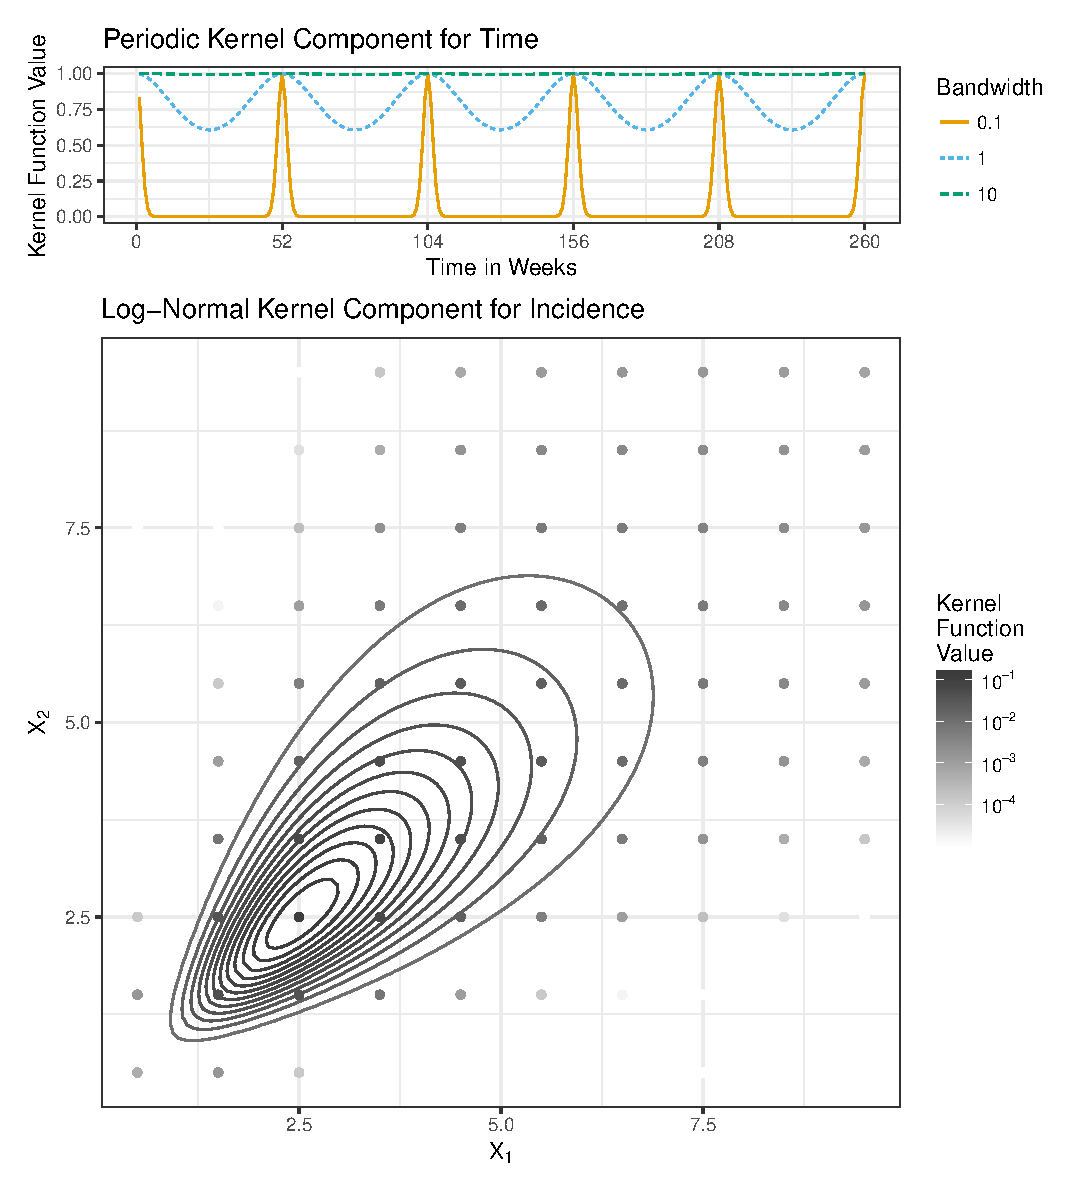
\includegraphics[width=\maxwidth]{figure/Fig1_Evan_L_Ray_KernelPlot-1} 

\end{knitrout}
\caption{The components of the kernel function.  The top panel shows the
periodic kernel function illustrated as a function of time in weeks with
$\rho = \pi / 52$ and three possible values for the bandwidth parameter
$\eta$.  The lower panel shows the log-normal kernel function in the bivariate
case.  The curves indicate contours of the continuous kernel function and the
points indicate the discrete kernel function, which is obtained by integrating
the continuous kernel function.  The kernel is centered at $(2.5, 2.5)$ and has
bandwidth matrix $\begin{bmatrix}0.2 & 0.15 \\ 0.15 & 0.2\end{bmatrix}$.}
\label{fig:PeriodicKernelPlot}
\end{figure}


\begin{figure}
\begin{knitrout}
\definecolor{shadecolor}{rgb}{0.969, 0.969, 0.969}\color{fgcolor}
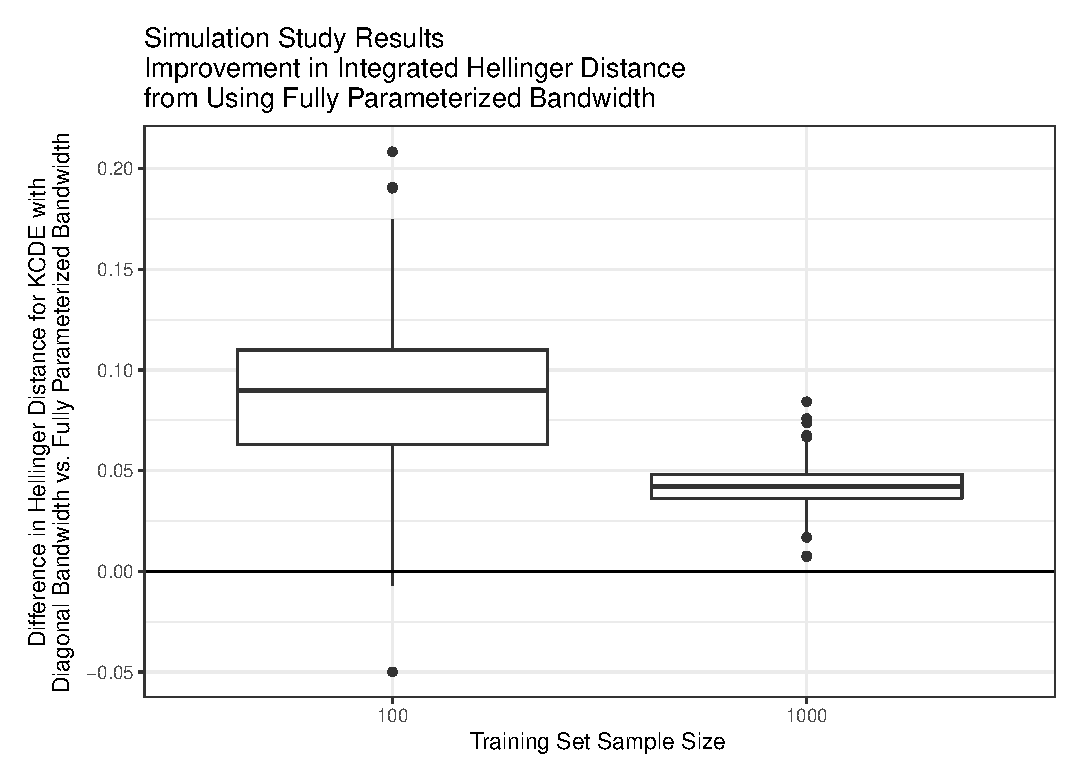
\includegraphics[width=\maxwidth]{figure/Fig2_Evan_L_Ray_SimStudyResultsPlot-1} 

\end{knitrout}
\caption{Box plots of results from the simulation study.  Positive values
indicate simulation trials where the full bandwidth specification outperformed the diagonal bandwidth
specification with the same training data set, as measured by Hellinger distance from the
target conditional density.}
\label{fig:SimStudyResultsPlot}
\end{figure}


\begin{figure}
\begin{knitrout}
\definecolor{shadecolor}{rgb}{0.969, 0.969, 0.969}\color{fgcolor}
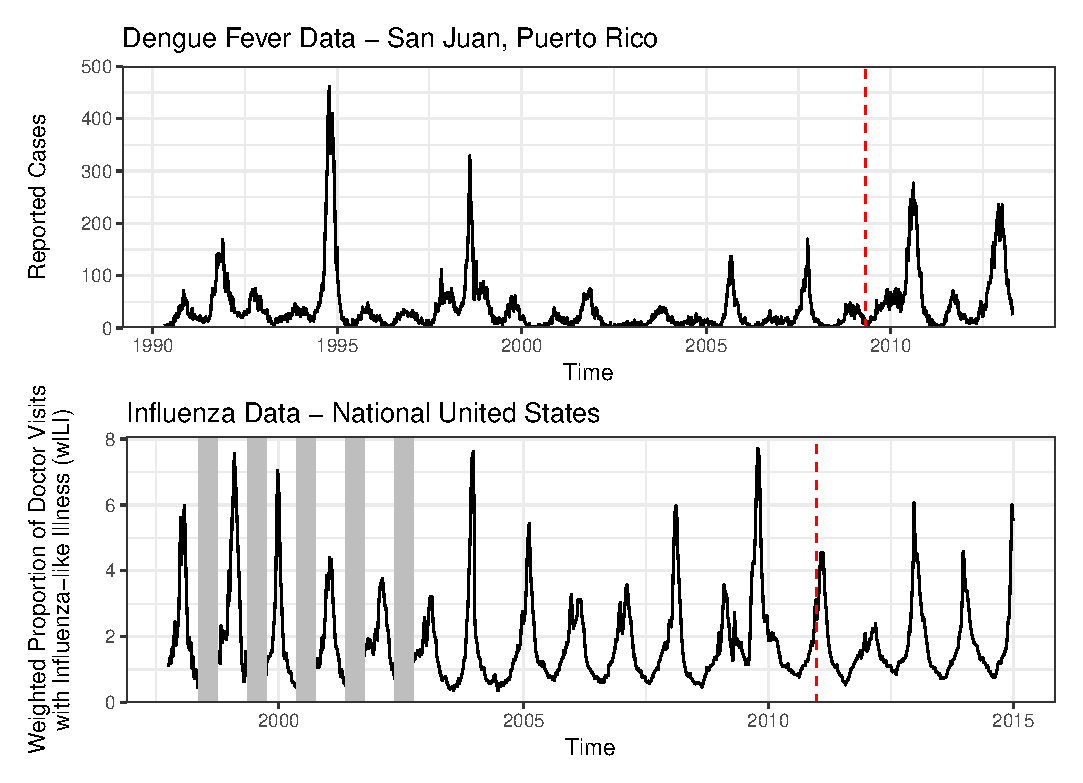
\includegraphics[width=\maxwidth]{figure/Fig3_Evan_L_Ray_InitialDataPlot-1} 

\end{knitrout}
\caption{Plots of the data sets we apply our methods to.  In each case, the last
four years of data are held out as a test data set; this cutoff is indicated
with a vertical dashed line.  For the flu data set, low-season incidence was not
recorded in early years of data collection.  These missing data are indicated
with vertical grey bars.}
\label{fig:IntialDataPlots}
\end{figure}

\begin{figure}
\begin{knitrout}
\definecolor{shadecolor}{rgb}{0.969, 0.969, 0.969}\color{fgcolor}
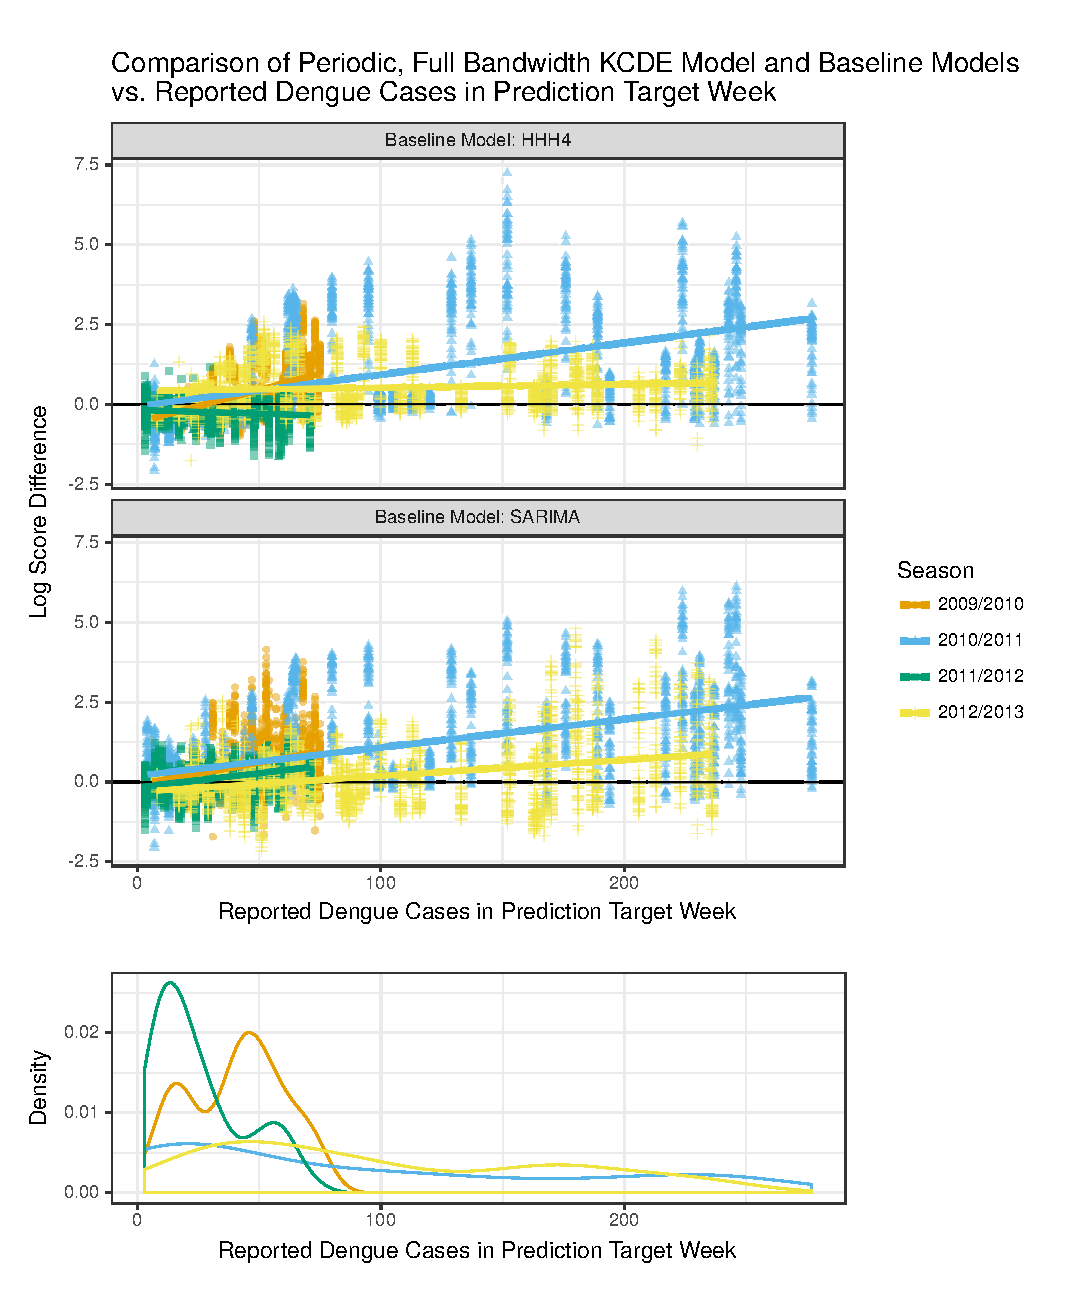
\includegraphics[width=\maxwidth]{figure/Fig4_Evan_L_Ray_DengueLogScoreDiffVsReportedCasesCombined-1} 

\end{knitrout}
\caption{Differences in log scores for the weekly predictive distributions
obtained from the Periodic, Full Bandwidth KCDE model and the baseline
models, plotted against the observed incidence in the week being predicted.
For reference, a log score difference of 2.3 (4.6) indicates that the predictive density from KCDE was about 10 (100)
times as large as the predictive density from the baseline model at the realized outcome.  Each
point corresponds to a unique combination of prediction target week and
prediction horizon.
The lower panel displays a density estimate of incidence levels in each week
of the season separately for each season in the test phase.
}
\label{fig:DengueLogScoreDiffVsReportedCasesCombined}
\end{figure}

\begin{figure}
\begin{knitrout}
\definecolor{shadecolor}{rgb}{0.969, 0.969, 0.969}\color{fgcolor}
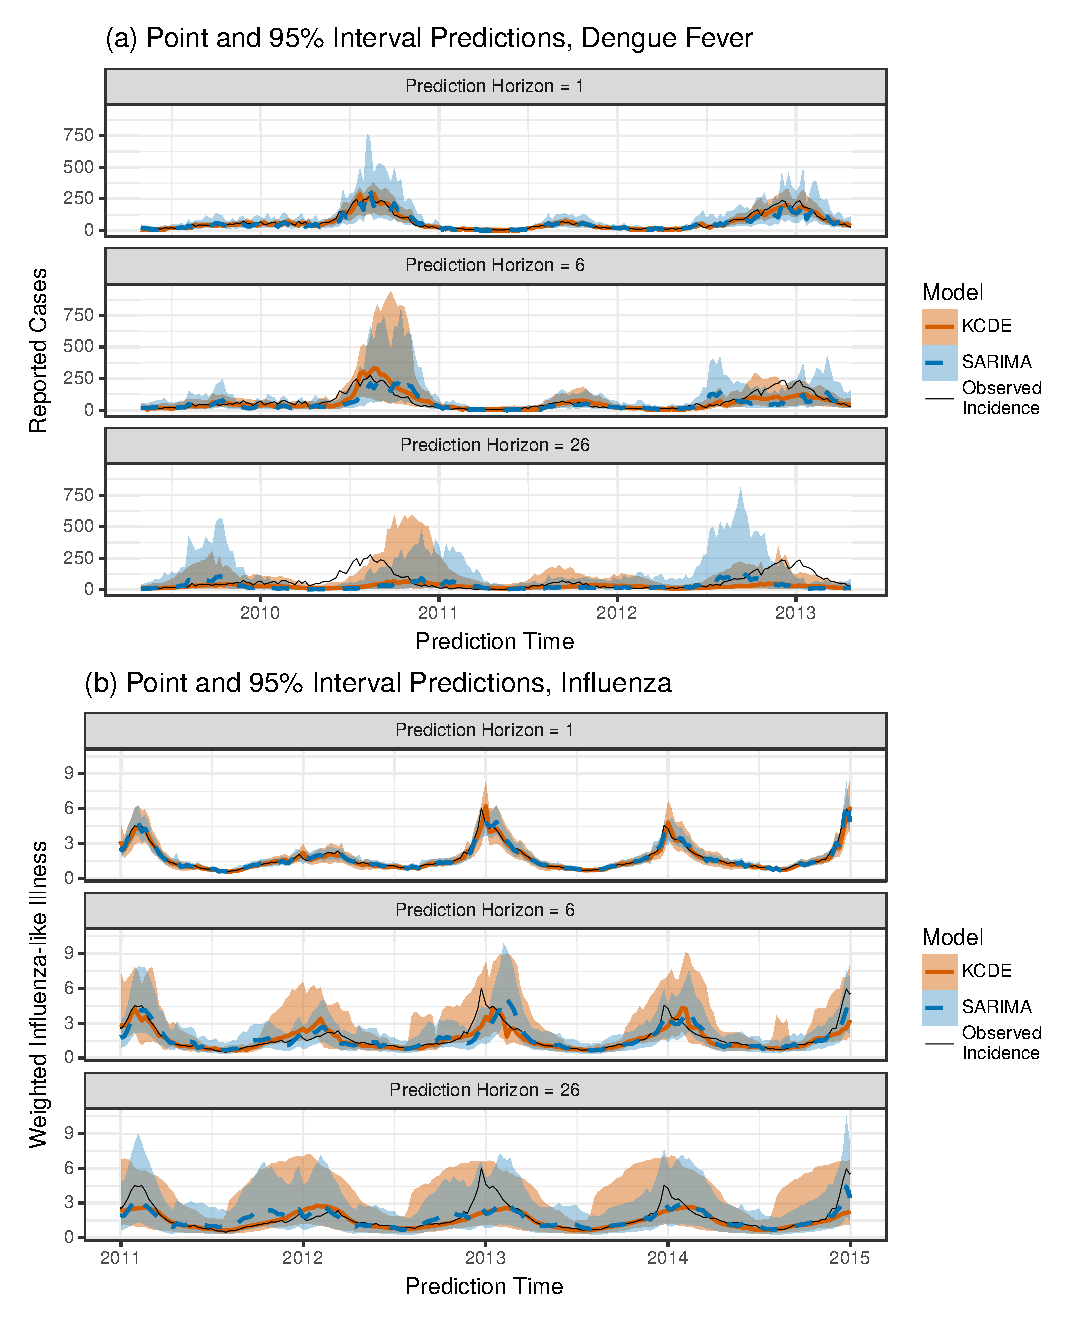
\includegraphics[width=\maxwidth]{figure/Fig5_Evan_L_Ray_DengueDataRibbonsPredictionPlot95Intervals-1} 

\end{knitrout}
\caption{Plots of point and interval predictions from SARIMA and the
Periodic, Full Bandwidth KCDE model.  The point prediction is the median of the predictive
distribution for incidence in the given week.  The interval prediction is a percentile interval; for example, the endpoints of the 95\% prediction interval are the 2.5th percentile and the 97.5th percentile of the predictive distribution.}
\label{fig:DengueRibbonsPredictions}
\end{figure}


\begin{table}[hp]
\begin{tabular}{lllll}
\toprule
         &          &              &    \multicolumn{2}{c}{Summary of Log Scores} \\
\cline{4-5}
 Disease & Subset & Model & Min & Mean \\
  \hline
Dengue & All Weeks & Null KCDE & -9.981 & -5.147\\
 &  & Full Bandwidth KCDE & -10.373 & -5.165\\
 &  & Periodic KCDE & -11.047 & -5.021\\
 &  & \textbf{Periodic, Full Bandwidth KCDE} & -10.851 & \textbf{-5.019}\\
 &  & \underline{\emph{HHH4}} & \underline{\emph{-16.201}} & -5.369\\
 &  & SARIMA & -14.416 & -5.456\\
\cline{2-5}
\cline{2-5}
 & High Incidence & Null KCDE & -9.981 & -8.235\\
 &  & Full Bandwidth KCDE & -10.373 & -8.339\\
 &  & Periodic KCDE & -11.047 & -7.841\\
 &  & \textbf{Periodic, Full Bandwidth KCDE} & -10.851 & \textbf{-7.791}\\
 &  & \underline{\emph{HHH4}} & \underline{\emph{-14.665}} & -9.046\\
 &  & SARIMA & -14.416 & -9.380\\
\midrule
Influenza & All Weeks & Null KCDE & -4.430 & -1.039\\
 &  & Full Bandwidth KCDE & -5.004 & -0.993\\
 &  & Periodic KCDE & -3.660 & -0.668\\
 &  & \textbf{Periodic, Full Bandwidth KCDE} & -3.850 & \textbf{-0.642}\\
 &  & \underline{\emph{SARIMA}} & \underline{\emph{-6.385}} & -0.666\\
\cline{2-5}
\cline{2-5}
 & High Incidence & Null KCDE & -4.430 & -2.887\\
 &  & Full Bandwidth KCDE & -5.004 & -3.025\\
 &  & Periodic KCDE & -3.660 & -2.404\\
 &  & Periodic, Full Bandwidth KCDE & -3.850 & -2.447\\
 &  & \textbf{\underline{\emph{SARIMA}}} & \underline{\emph{-6.385}} & \textbf{-2.345}\\

\bottomrule
\end{tabular}
\caption{Summaries of model performance for predictions of incidence in individual weeks.
The ``All Weeks'' group summarizes log scores for all combinations of prediction horizon and target week in the test period;
the ``High Incidence" group summarizes log scores for predictions of indience in weeks where the
observed incidence was at least two thirds of the maximum weekly incidence in the test period.
The model in \textbf{bold} font
had the highest mean log score within each combination of disease and weeks subset.  The model in \underline{\emph{italicized and underlined}} font had the lowest minimum log score within each combination of disease and weeks subset.  In some cases, the same model had both the highest average log score and the lowest worst-case log score.
}
\label{tbl:IndWeeksIncidenceResults}
\end{table}



\begin{table}[ht]
\centering
\begin{tabular}{llll}
\toprule
         &       & \multicolumn{2}{c}{Nominal Coverage}   \\
\cline{3-4}
 Disease & Model & 50\% & 95\% \\
  \hline
Dengue & Null KCDE & 40.958 & \textbf{91.827}\\
 & Full Bandwidth KCDE & 38.794 & 89.571\\
 & Periodic KCDE & \textbf{44.749} & 87.343\\
 & Periodic, Full Bandwidth KCDE & 41.901 & 86.418\\
 & HHH4 & 40.163 & 78.217\\
 & SARIMA & 38.637 & 79.919\\
\cline{1-4}
Influenza & Null KCDE & \textbf{69.580} & 99.457\\
 & Full Bandwidth KCDE & 70.896 & 99.420\\
 & Periodic KCDE & 77.374 & 99.678\\
 & Periodic, Full Bandwidth KCDE & 76.150 & 99.485\\
 & SARIMA & 73.270 & \textbf{99.384}\\

\bottomrule
\end{tabular}
\caption{Coverage rates for predictions of disease incidence in individual weeks during the test time frame.  For each model specification, we have obtained the overall proportion of predictive intervals that contained the realized outcome, combining across all prediction horizons and all times in the test period at which the prediction was made.  For each combination of disease and target coverage rate, the result for the model with actual coverage rate closest to the target coverate rate is highlighted.}
\label{tbl:CoverageResults}
\end{table}


\begin{figure}
\begin{knitrout}
\definecolor{shadecolor}{rgb}{0.969, 0.969, 0.969}\color{fgcolor}
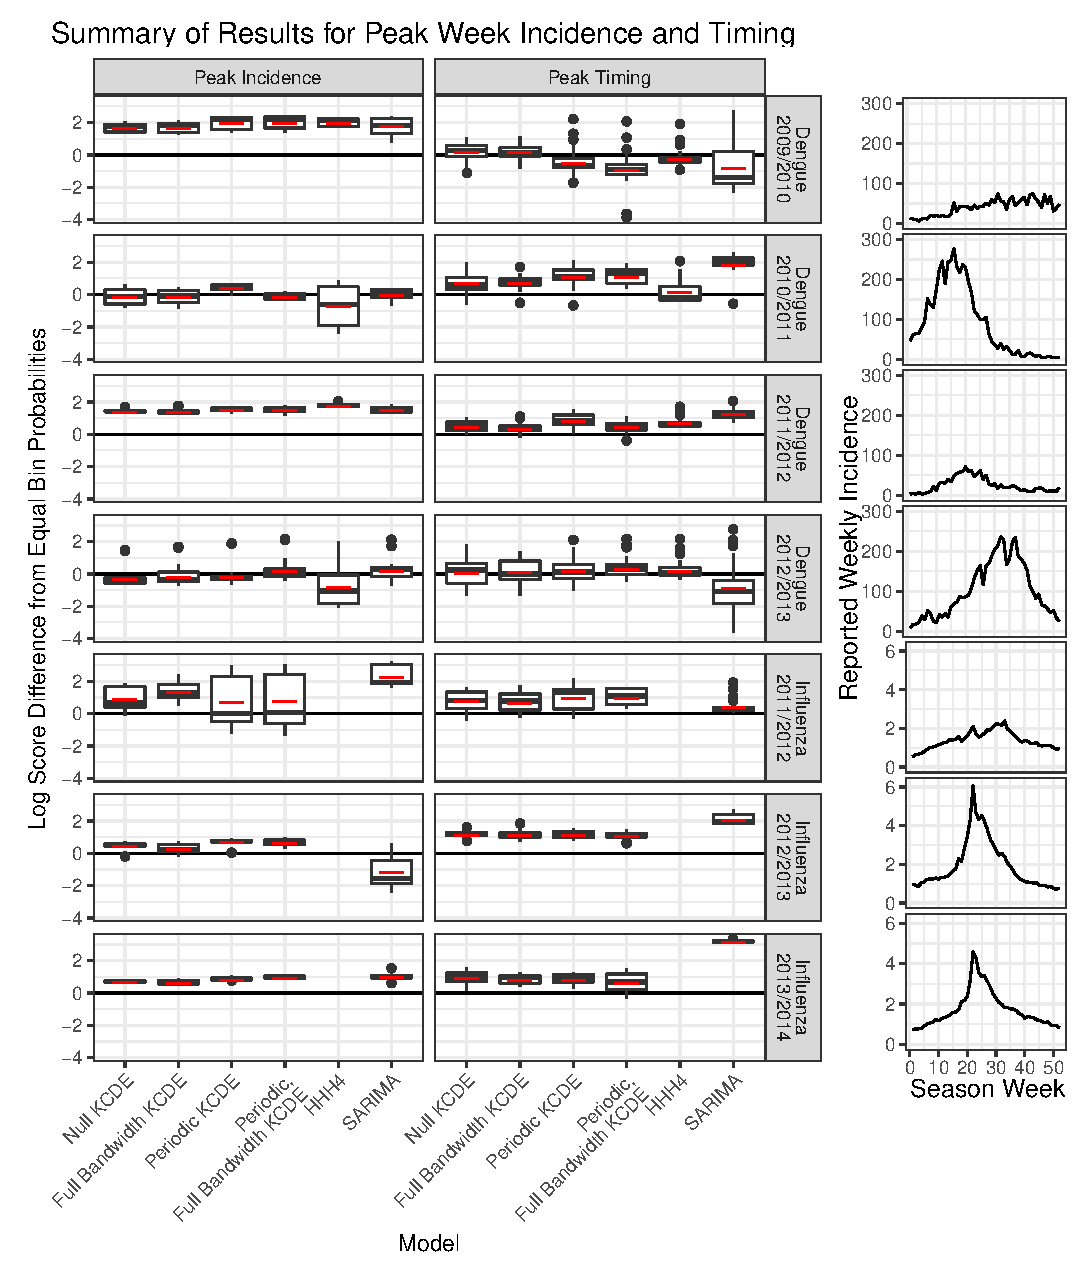
\includegraphics[width=\maxwidth]{figure/Fig6_Evan_L_Ray_PeakIncidenceLogScoreDiffFromEqualBoxplots-1} 

\end{knitrout}
\caption{A summary of performance of each method for predicting incidence in the peak week and
peak week timing.  Each boxplot summarizes all predictions made by a method in a given
season in weeks before the actual peak week for that season.  The vertical
axis is the difference in log scores between the given method and a naive approach assigning
equal probability to each week of the year.  Positive values indicate cases when
the method did better than using equal bin probabilities.  The horizontal red dash
indicates the mean log score for those predictions made before the peak within each season.
The plots on the right display the trajectory of incidence over each season.  There were
42 weeks before the peak in the 2009/2010 dengue season, 15 in the 2010/2011 dengue season,
19 in the 2011/2012 dengue season, 31 in the 2012/2013 dengue season,
23 in the 2011/2012 influenza season, and 12 in each of the 2012/2013 and 2013/2014 influenza seasons.
}
\label{fig:CombinedPeakWeekTimingPredictionLogScores}
\end{figure}



\begin{table}[hp]
\centering
\begin{tabular}{lllll}
\toprule
         &                    &          &              \multicolumn{2}{c}{Summary of Log Scores} \\
\cline{4-5}
 Disease & Subset & Model & Min & Mean \\
  \hline
Dengue & All Weeks & Null KCDE & -3.221 & -0.973\\
 &  & Full Bandwidth KCDE & -3.239 & -0.933\\
 &  & Periodic KCDE & -3.037 & -0.771\\
 &  & \textbf{Periodic, Full Bandwidth KCDE} & -2.802 & \textbf{-0.739}\\
 &  & \underline{\emph{HHH4}} & \underline{\emph{-4.816}} & -0.901\\
 &  & SARIMA & -3.088 & -0.836\\
 &  & Equal Bin Probabilities & -2.398 & -2.398\\
\cline{2-5}
 & Before Peak & Null KCDE & -3.221 & -1.570\\
 &  & Full Bandwidth KCDE & -3.239 & -1.531\\
 &  & Periodic KCDE & -3.037 & -1.315\\
 &  & \textbf{Periodic, Full Bandwidth KCDE} & -2.802 & \textbf{-1.282}\\
 &  & \underline{\emph{HHH4}} & \underline{\emph{-4.816}} & -1.600\\
 &  & SARIMA & -3.088 & -1.361\\
 &  & Equal Bin Probabilities & -2.398 & -2.398\\
\midrule
Influenza & All Weeks & Null KCDE & -3.487 & -1.423\\
 &  & Full Bandwidth KCDE & -3.483 & -1.311\\
 &  & Periodic KCDE & -4.528 & -1.337\\
 &  & Periodic, Full Bandwidth KCDE & -4.678 & -1.313\\
 &  & \textbf{\underline{\emph{SARIMA}}} & \underline{\emph{-5.714}} & \textbf{-1.140}\\
 &  & Equal Bin Probabilities & -3.296 & -3.296\\
\cline{2-5}
 & Before Peak & Null KCDE & -3.487 & -2.538\\
 &  & Full Bandwidth KCDE & -3.483 & -2.363\\
 &  & Periodic KCDE & -4.528 & -2.518\\
 &  & Periodic, Full Bandwidth KCDE & -4.678 & -2.471\\
 &  & \textbf{\underline{\emph{SARIMA}}} & \underline{\emph{-5.714}} & \textbf{-2.190}\\
 &  & Equal Bin Probabilities & -3.296 & -3.296\\

\bottomrule
\end{tabular}
\caption{Summaries of model performance for predictions of incidence in the peak week.
The ``All Weeks'' group summarizes results for all combinations of
target week in the test period and prediction horizon; the ``Before Peak" group summarizes results
for predictions in weeks before the actual peak for the given season.  The model in \textbf{bold} font
had the highest mean log score within each combination of disease and weeks subset.  The model in \underline{\emph{italicized and underlined}} font had the lowest minimum log score within each combination of disease and weeks subset.  In some cases, the same model had both the highest average log score and the lowest worst-case log score.
There were 42 weeks before the peak in the 2009/2010 dengue season, 15 in the 2010/2011 dengue season,
19 in the 2011/2012 dengue season, 31 in the 2012/2013 dengue season,
23 in the 2011/2012 influenza season, and 12 in each of the 2012/2013 and 2013/2014 influenza seasons.}
\label{tbl:PeakIncidenceResults}
\end{table}



\begin{table}[hp]
\centering
\begin{tabular}{lllll}
\toprule
         &                    &          &              \multicolumn{2}{c}{Summary of Log Scores} \\
\cline{4-5}
 Disease & Subset & Model & Min & Mean \\
  \hline
Dengue & All Weeks & Null KCDE & -5.298 & -2.135\\
 &  & Full Bandwidth KCDE & -5.279 & -2.116\\
 &  & \textbf{Periodic KCDE} & -5.684 & \textbf{-2.107}\\
 &  & \underline{\emph{Periodic, Full Bandwidth KCDE}} & \underline{\emph{-7.824}} & -2.197\\
 &  & HHH4 & -4.867 & -2.115\\
 &  & SARIMA & -7.601 & -2.297\\
 &  & Equal Bin Probabilities & -3.951 & -3.951\\
\cline{2-5}
 & Before Peak & \textbf{Null KCDE} & -5.298 & \textbf{-3.645}\\
 &  & Full Bandwidth KCDE & -5.279 & -3.656\\
 &  & Periodic KCDE & -5.684 & -3.759\\
 &  & \underline{\emph{Periodic, Full Bandwidth KCDE}} & \underline{\emph{-7.824}} & -3.940\\
 &  & HHH4 & -4.867 & -3.814\\
 &  & SARIMA & -7.601 & -4.001\\
 &  & Equal Bin Probabilities & -3.951 & -3.951\\
\midrule
Influenza & All Weeks & \underline{\emph{Null KCDE}} & \underline{\emph{-4.374}} & -1.689\\
 &  & Full Bandwidth KCDE & -4.193 & -1.708\\
 &  & Periodic KCDE & -4.227 & -1.568\\
 &  & Periodic, Full Bandwidth KCDE & -4.283 & -1.601\\
 &  & \textbf{SARIMA} & -3.868 & \textbf{-1.258}\\
 &  & Equal Bin Probabilities & -3.951 & -3.951\\
\cline{2-5}
 & Before Peak & \underline{\emph{Null KCDE}} & \underline{\emph{-4.374}} & -3.014\\
 &  & Full Bandwidth KCDE & -4.193 & -3.094\\
 &  & Periodic KCDE & -4.227 & -2.945\\
 &  & Periodic, Full Bandwidth KCDE & -4.283 & -3.000\\
 &  & \textbf{SARIMA} & -3.868 & \textbf{-2.383}\\
 &  & Equal Bin Probabilities & -3.951 & -3.951\\

\bottomrule
\end{tabular}
\caption{Summaries of model performance for predictions of peak week timing.
The ``All Weeks'' group summarizes results for all combinations of
target week in the test period and prediction horizon; the ``Before Peak" group summarizes results
for predictions in weeks before the actual peak for the given season.  The model in \textbf{bold} font
had the highest mean log score within each combination of disease and weeks subset.  The model in \underline{\emph{italicized and underlined}} font had the lowest minimum log score within each combination of disease and weeks subset.  In some cases, the same model had both the highest average log score and the lowest worst-case log score.
There were 42 weeks before the peak in the 2009/2010 dengue season, 15 in the 2010/2011 dengue season,
19 in the 2011/2012 dengue season, 31 in the 2012/2013 dengue season,
23 in the 2011/2012 influenza season, and 12 in each of the 2012/2013 and 2013/2014 influenza seasons.}
\label{tbl:PeakTimingResults}
\end{table}

\end{document}
